\documentclass[12pt, oneside, letterpaper]{book}
\usepackage{tree-dvips}
\usepackage{lingmacros}
\usepackage[utf8]{inputenc}
\usepackage[spanish]{babel}
\usepackage{graphicx}
\usepackage{subcaption}
\usepackage{hyperref}

\begin{document}
%%%%%%%%%%%%%   NOMBRE DEL PROYECTO  %%%%%%5
\title{\textbf{"Friends Night"}: Documento de Requerimentos}

\author{\textbf{COR Studios}\\Luis Lemus\\Víctor Sánchez\\ Diego Lecanda\\André Cerdán}


\maketitle
\newpage
\frontmatter
%\section*{Indice}
\tableofcontents{}

\newpage
\mainmatter
%%%%%%%%%%%%%% INTRODUCCION %%%%%%
\part{Introducción}
%%% DESCRIOCUON DEL PROYECTO %%%%%%%%%%%
\chapter{Descripción del proyecto}
\par
Esta aplicación es un videojuego de fiesta o ''party game'' el cual busca brindar distintos juegos para que la gente en las fiestas pueda jugar entre ellos, usando la pantalla únicamente para ver instrucciones y algunas dinámicas del juego, además de que permitirá usar filtros para buscar juegos que se acomoden a la situación, ya sea por cantidad de jugadores, gustos, materiales necesarios y algunos otros. En resumen nuestra aplicación sera un videojuego que sirva como puente para que los jóvenes puedan convivir y jugar. 

%%%%%%%%%%%5
\chapter{Entender al usuario}
\par Para entender mejor al usuario o jugador que comprará o usará nuestra app realizamos un empathy map y tres ''Buyer person'' es decir, 3 modelos de lo que sería nuestro comprador ideal, alguien que quizás compre el juego y el que no lo compraría, además, también hicimos un User Journey Map para identificar lo que siente, piensa, considera y hace a lo largo del proceso desde buscar y bajar el juego hasta compartirlo una vez jugado.
%%% Empathy map %%
\par 
Primero, tenemos el empathy map, tanto la plantilla que usamos como las observaciones que hicimos
\begin{figure}[h]
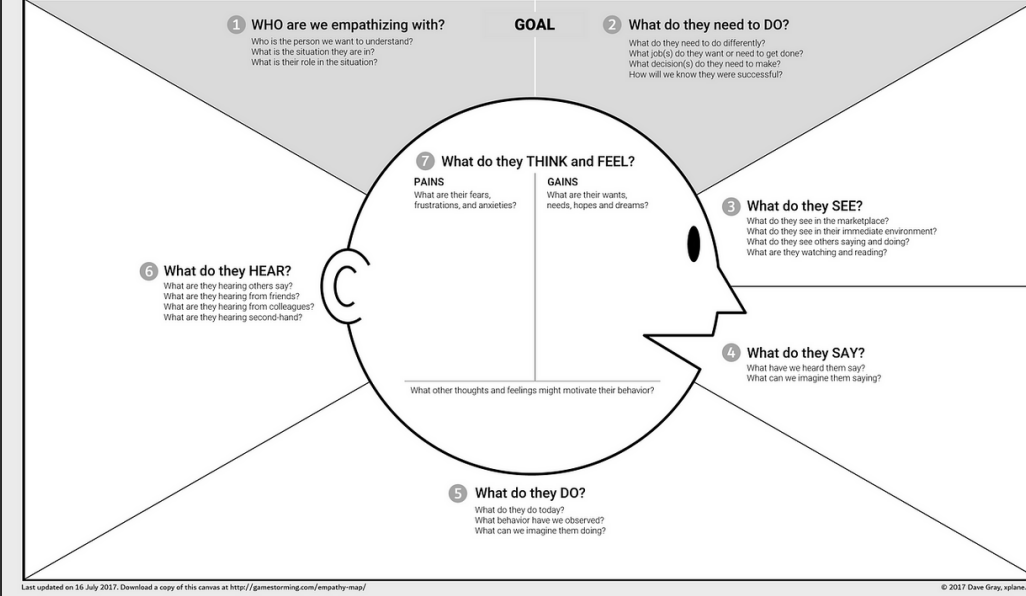
\includegraphics[width=1.2\columnwidth]{EMcaraFN.png}%
\caption{Base del empathy map usado }%
\label{BaseEMFN}%
\end{figure}

\begin{figure}[h]
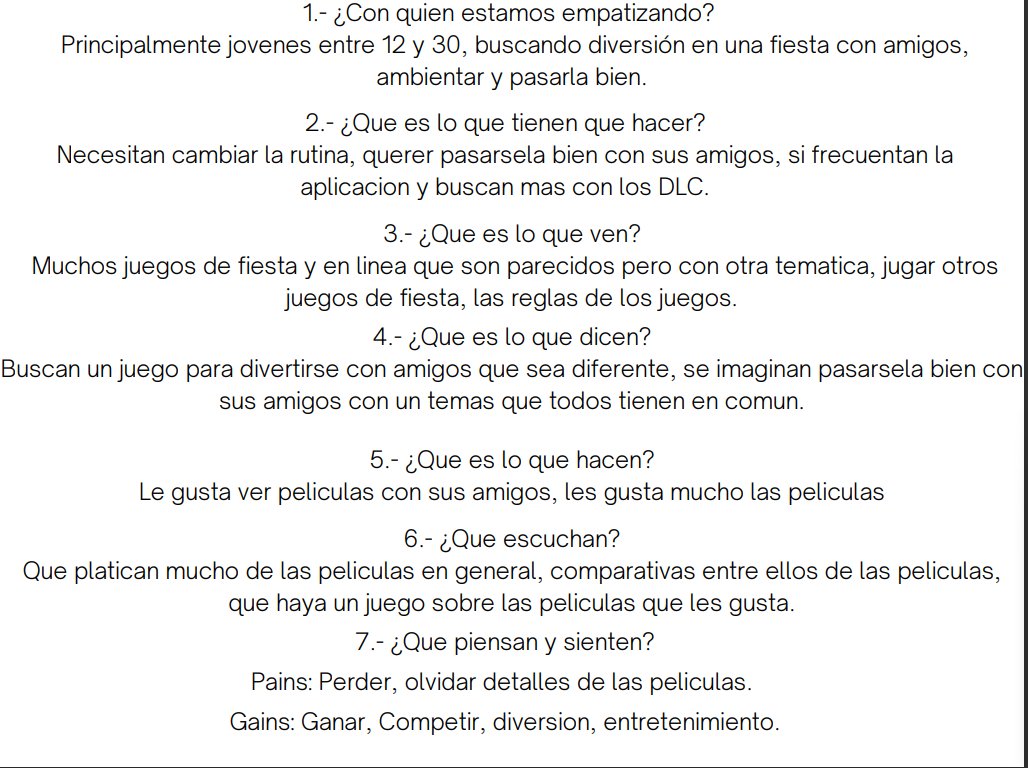
\includegraphics[width=1.2\columnwidth]{EMexplicacionFN.png}%
\caption{Observaciones del empathy map }%
\label{EMFN}%
\end{figure}
%%%%%%%%%%%%%%%%%%%%
\par Después tenemos el User Journey Map 
\begin{figure}[h]
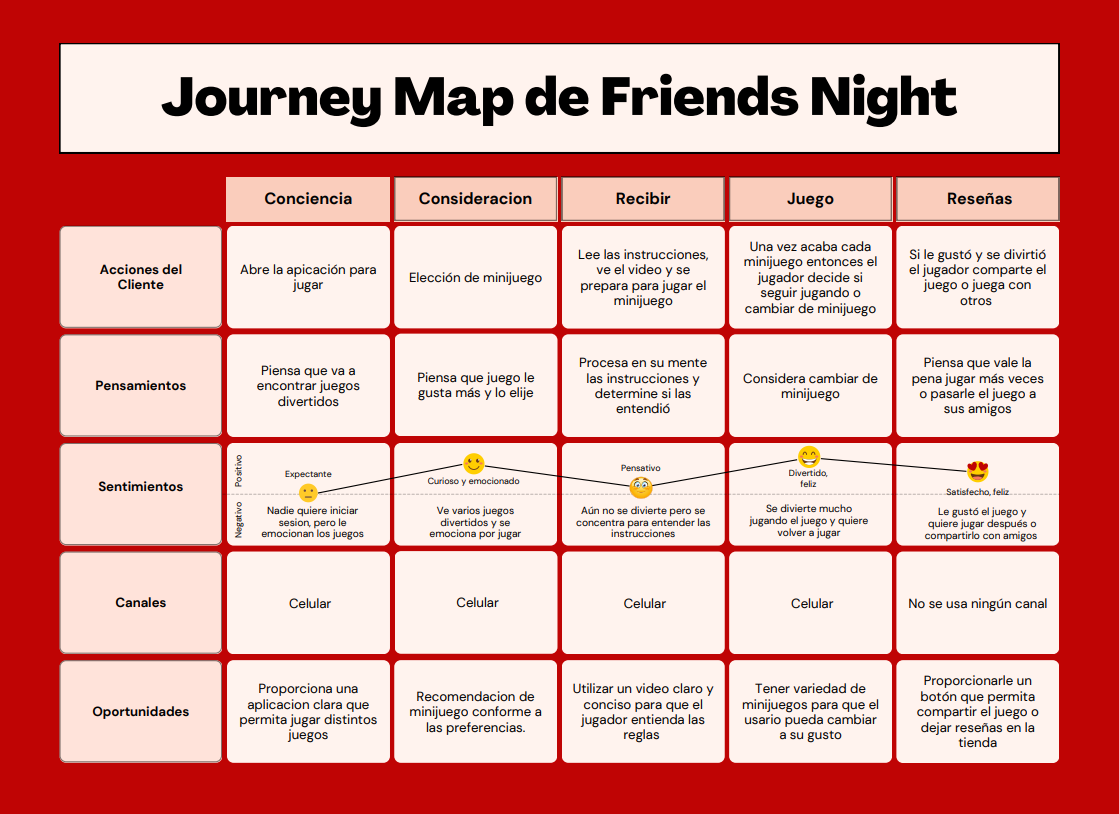
\includegraphics[width=1.2\columnwidth]{UserJourneyMapFN.png}%
\caption{User Journey Map }%
\label{UJMFN}%
\end{figure}
%%%%%%%%%%%
\par Además, contamos con tres tipos de compradores, el que seguro compraría el juego, el que tal vez lo haría y el que no lo haría (En ese orden):
\begin{figure}[h]
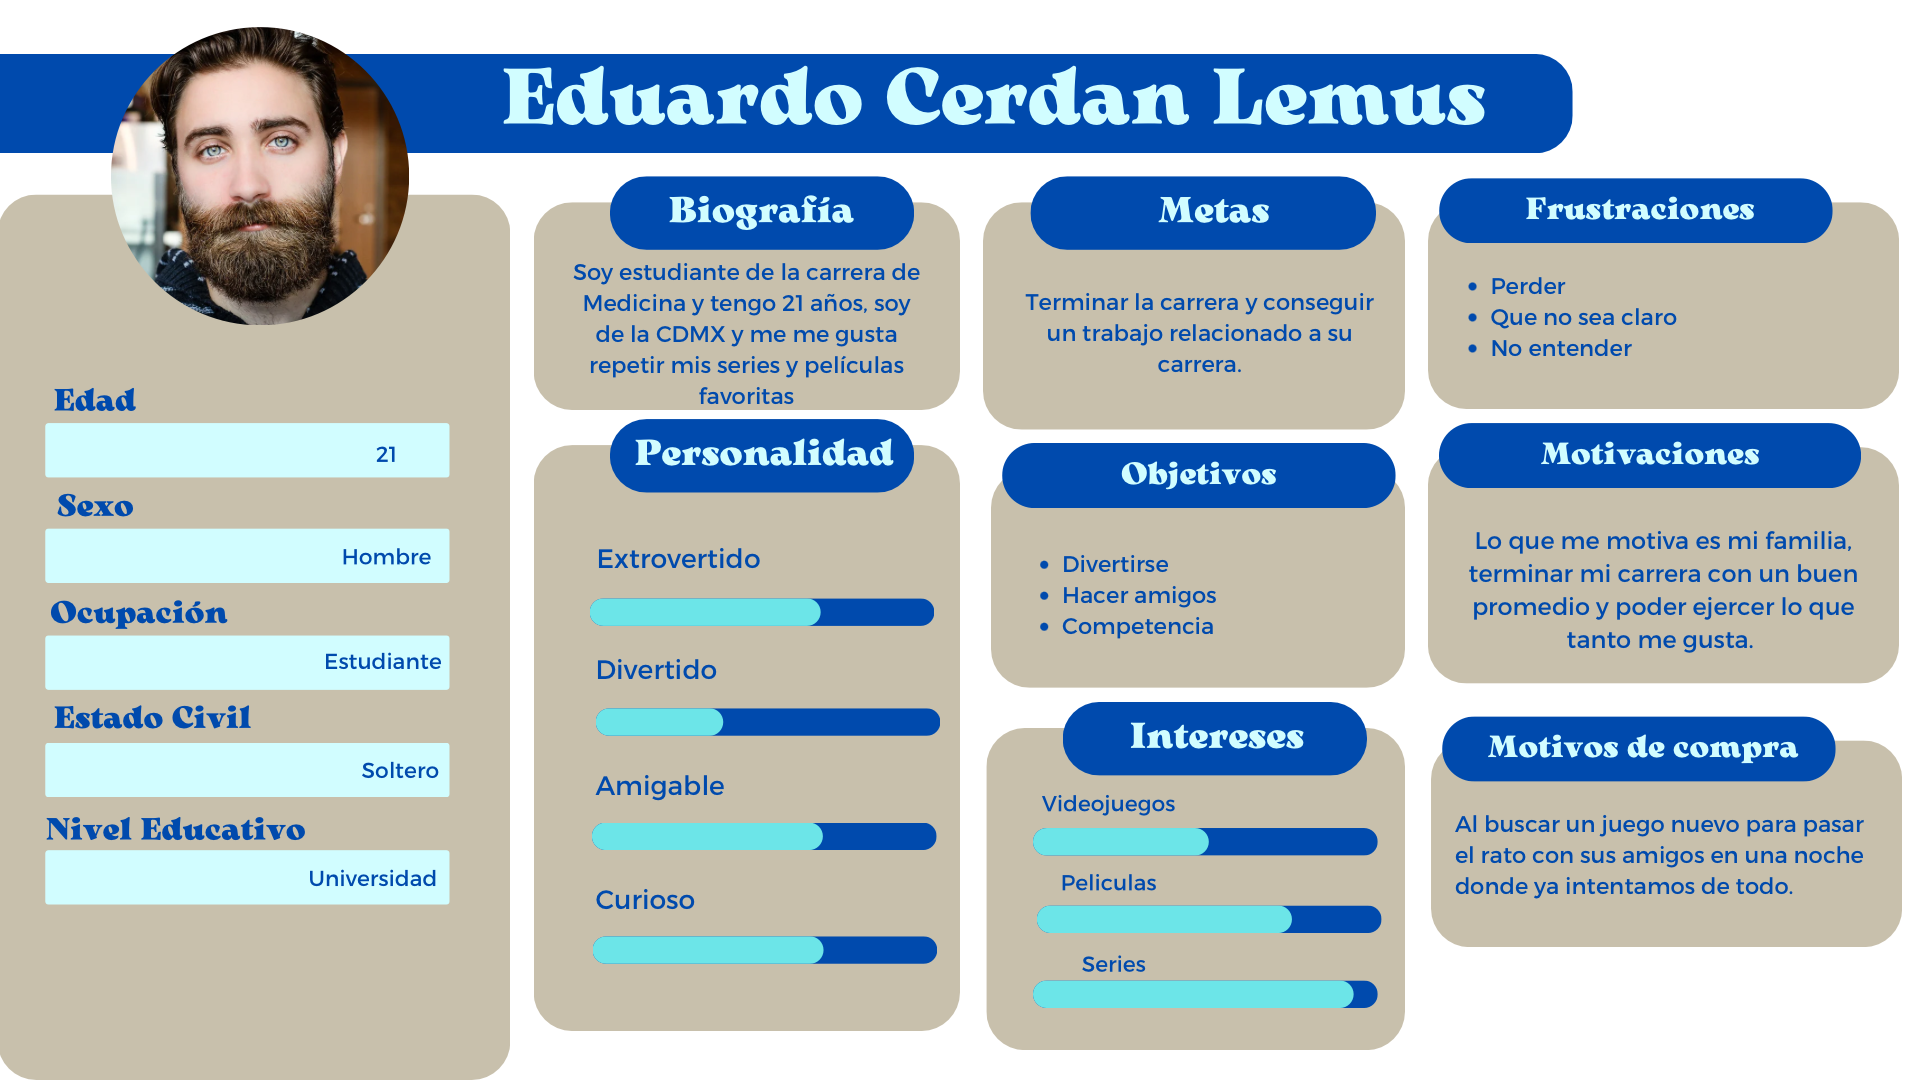
\includegraphics[width=1.2\columnwidth]{IdealBuyerFN.png}%
\caption{Ideal Buyer }%
\label{IBFN}%
\end{figure}

\begin{figure}[h]
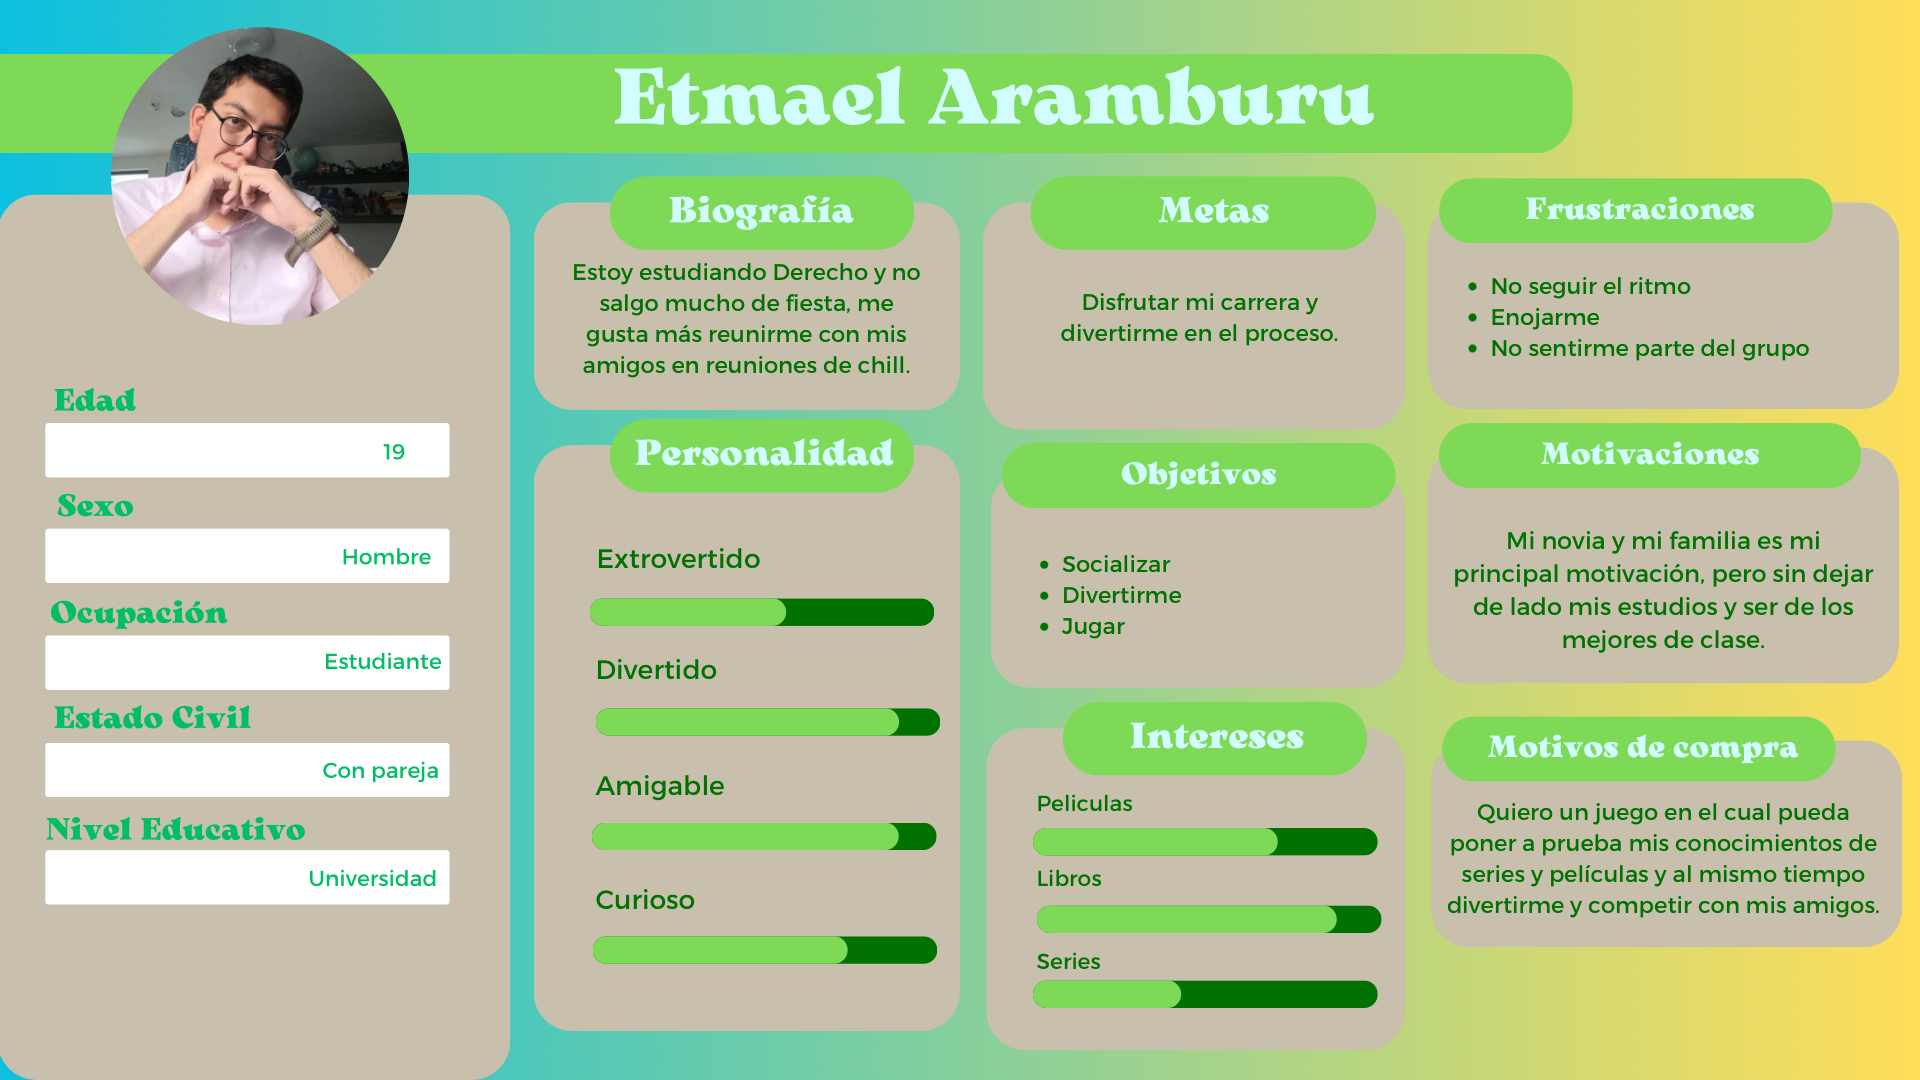
\includegraphics[width=1.2\columnwidth]{MehIdealBuyerFN.png}%
\caption{Buyer que quizás compraría el juego}%
\label{MBFN}%
\end{figure}

\begin{figure}[h]
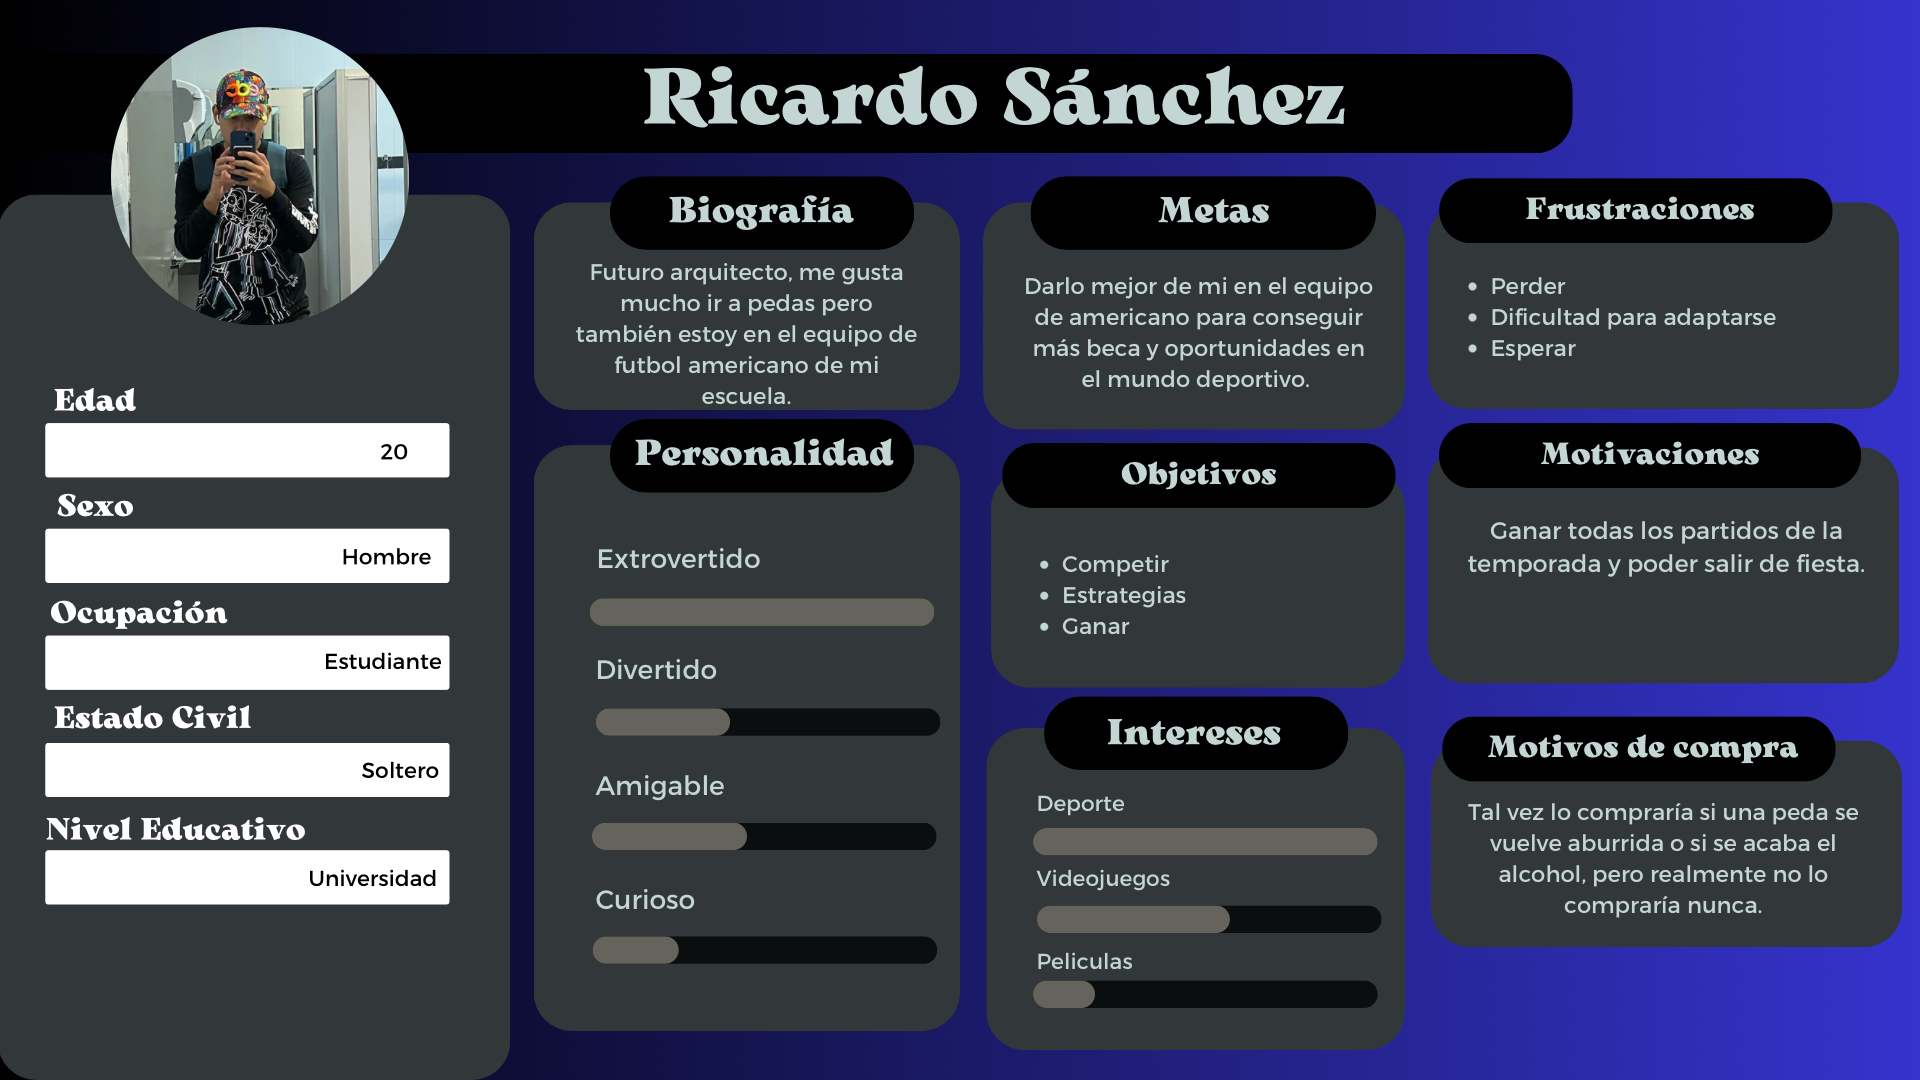
\includegraphics[width=1.2\columnwidth]{NotIdealBuyerFN.png}%
\caption{User Journey Map }%
\label{NIBFN}%
\end{figure}

%%%%%%%%%%%%%
\part{Requerimentos y diagramas}

%%%%%%%%%%%%%% REQUERIMENTOS FUNCIONALES %%%%%%%%%%%%%%%%%55
\chapter{Requerimentos funcionales}
\fontsize{14}{18}\selectfont
Los requerimientos funcionales de la aplicación \textbf{Friends Night} son:
\par 
\begin{enumerate}
\item Crear un perfil
\item Administrar perfil 
\item Cambiar imagen de perfil
\item Cambiar nombre del perfil 
\item Filtro de contenido por edad
\item Preferencias de generos de película 
\item Enviar queja o comentario al soporte técnico
\item Ajustar el rendimiento en el dispositivo
\item Editar el perfil
\item Buscar juegos por categorías
\item Elegir un juego
\item Jugar el juego
\item Acceder al menu de opciones
\item Regresar al menu principal 
\end{enumerate}
%%%%%%%%%%%  REQUERIMENTOS NO FUNCIONALES %%%%%%%%%%%%%%%%%%%%55
%nota mental: puedo poner espacios con \bigskip o con \vspace{1cm} ...  \bigskip es irónicamente más pequeño

\chapter{Requerimentos no funcionales}
\fontsize{14}{18}\selectfont
\par 
\section{Requerimentos de usabilidad: }
\begin{enumerate}
\item Interfaz clara que permita ver donde hay ajustes y donde es para jugar (sobre todo para usuarios no acostumbrados a la tecnología).
\end{enumerate}

\section{Requerimentos de desarrollo: }
\begin{enumerate}
\item Trabajar con sistemas operativos de window 10 o mayor (Abstenerse de usar sistemas IOS). 
\item Las imagenes solo se podrán cambiar entre las predeterminadas, no subir ninguna más.
\end{enumerate}

\section{Requerimentos de entorno/de software: }
\begin{enumerate}
\item Sistemas Ios y Android

\end{enumerate}

\section{Requerimentos de eficiencia: }
\begin{enumerate}
\item La aplicación no debe tardar mucho tiempo en conectar a los jugadores entre ellos.
\end{enumerate}

\section{Requerimentos de disponibilidad: }
\begin{enumerate}
\item Mostrar desde el área de descarga la compatibilidad con dispositivos Android e IOS
\end{enumerate}

\section{Requerimentos de mantenimiento: }
\begin{enumerate}
\item Version de unity 2021.3.8f LTS con mantenimiento de 3 años desde que salió 
\end{enumerate}

\section{Requerimentos regulatorios: }
\begin{enumerate}
\item Acatar regulaciones respecto a contenido +18 respecto a consumo de alcohol 
\end{enumerate}

\section{Requerimentos éticos }
\begin{enumerate}
\item Advertir acerca de los juegos +18 de bebida, tanto en la página donde se publique el juego como dentro del juego
\end{enumerate}

%%%%%%%%%%%  ARQUITECTURA  %%%%%%%%%%
\newpage 
\chapter{Arquitectura}  

\p La arquitectura que escogimos para el proyecto es la arquitectura de Modelo-Vista-Controlador (también conocida por su abreviacion como MVC). Esta arquitectura consiste en una programación y acomodo del sistema en tres partes: La vista, donde se habla literalmente de la interfaz que vemos, la cual sera realizada en unity para este proyecto con ayuda de los elementos de unity hechos en C# donde lo procesado por el controlador se le muestre al usuario; El controlador son los códigos que literalmente controlan el programa, así, en este caso se manejará en unity con códigos en C# y en algunos casos códigos de PHP o similares que controlarán solicitudes de creación de cuenta o similares, en este caso se hará a través de alguna API o de algun método que permita conectar la vista del usuario y el modelo; Por último, el modelo, el cúal será una base de datos en Firebase o SQLite o algun otro sistema de bases de datos que nos permita conectarnos con unity.

%%%%%%% DIAGRAMAS  %%%%%%%%%
\chapter{Diagramas}
\newpage
%%%%%%% DIAGRAMAS DE CASOS DE USO %%%%%%%%%

\section{Diagrama de casos de uso}
\begin{figure}[h]
    \begin{flushleft}
        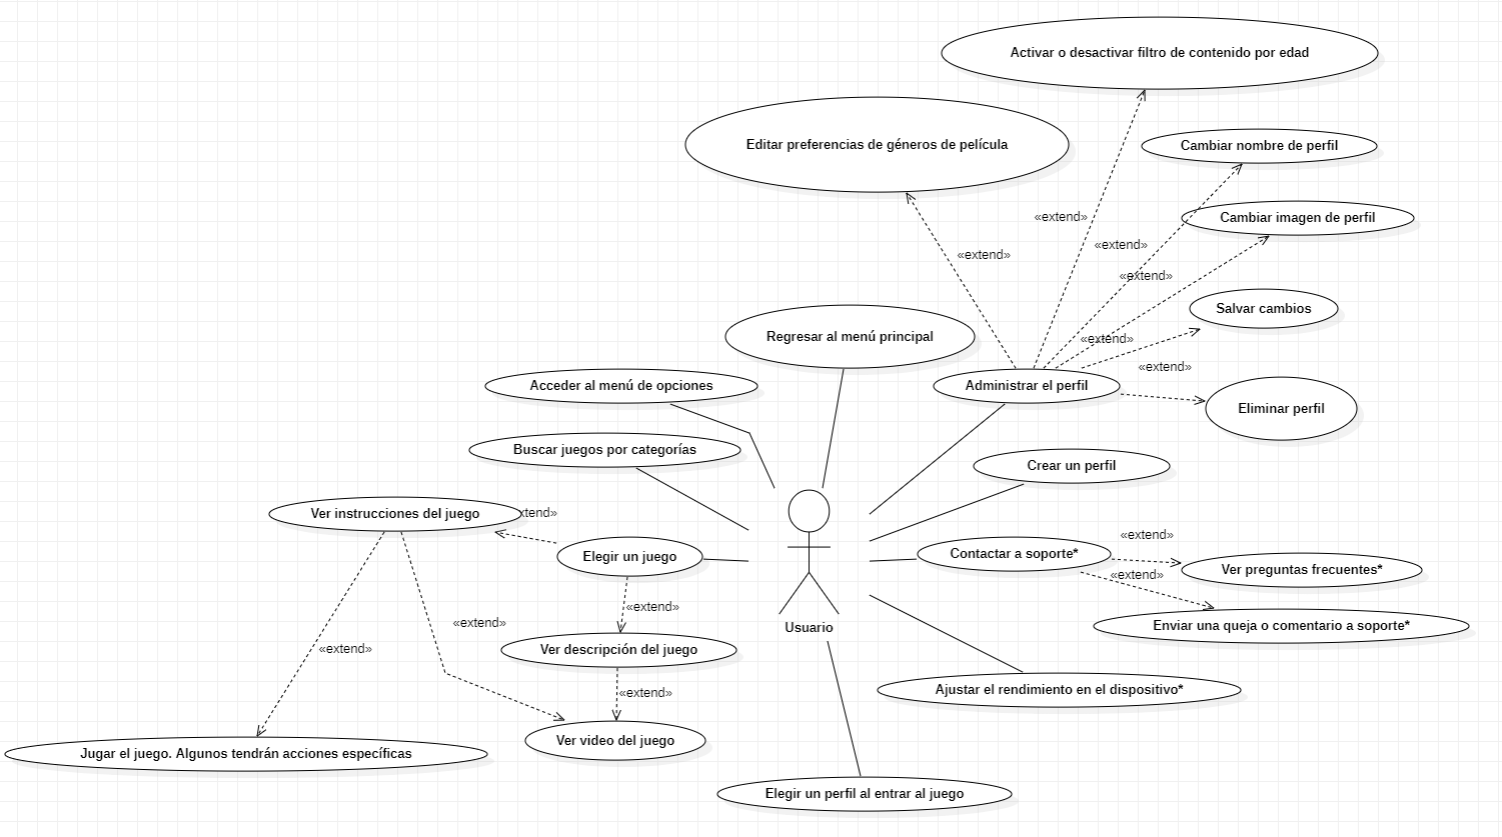
\includegraphics[width=1.1\textwidth]{DiagramaUsoDeCasoFN.png}
        \caption{Diagrama de uso de caso}
        \label{Diagrama}
    \end{flushleft}
\end{figure}


\vspace{1cm}

%%%%%%%%%%%%%%%%%%%%%%%%%%%%%%
\section{Diagrama de componentes}
\fontsize{14}{18}\selectfont
\par 
El siguiente diagrama de componentes de \textbf{Friends Night} contempla la arquitectura con la que se conectaran la base de datos, el juego y el usuario

\begin{center}
	\centering
		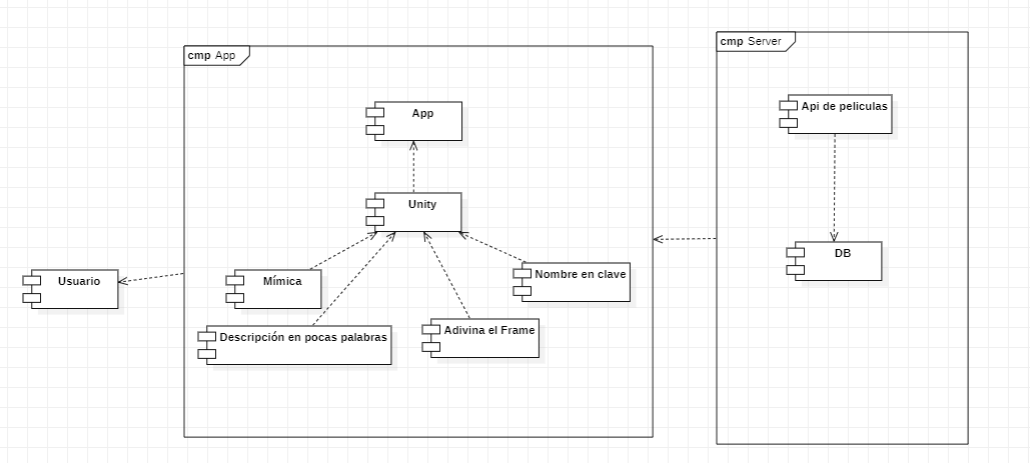
\includegraphics[width=1.2\textwidth]{DiagramaDeComponentesFriendsNight.png}

	\caption{Diagrama de componentes}
	\label{DiagramaComponentes}
\end{center}
\vspace{1cm}
%%%%%%%%%%%DIAGRAMA DE BASES DE DATOS ENTIDAD RELACION%%%%%%%%%%%%%%

\section{Diagrama de Bases de Datos \textit{Entidad Relación} }
\fontsize{14}{18}\selectfont
\par 
El siguiente diagrama de Entidad Relación \textbf{Friends Night} contempla las distintas entidades que necesitaran guardar información en la base de datos:

\begin{center}
	\centering
		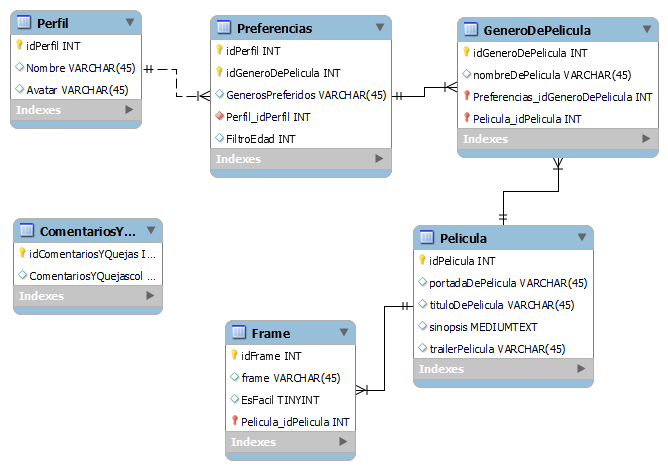
\includegraphics[width=1.2\textwidth]{DiagramaEntidadRelacionFriendsNight.png}

	\caption{Diagrama de bases de datos entidad relación}
	\label{DiagramaBasesDeDatos}
\end{center}
\vspace{1cm}
%nota mental: puedo poner espacios con \bigskip o con \vspace{1cm} ...  \bigskip es irónicamente más pequeño
%%%%%%%%%%%%%%%%%%%%%%%%%%%%%%

\section{Diagrama de Clases }
\fontsize{14}{18}\selectfont
\par 
El siguiente diagrama de clases de \textbf{Friends Night} contempla las distintas clases que se programarán en el desarrollo del juego:

\begin{center}
	\centering
		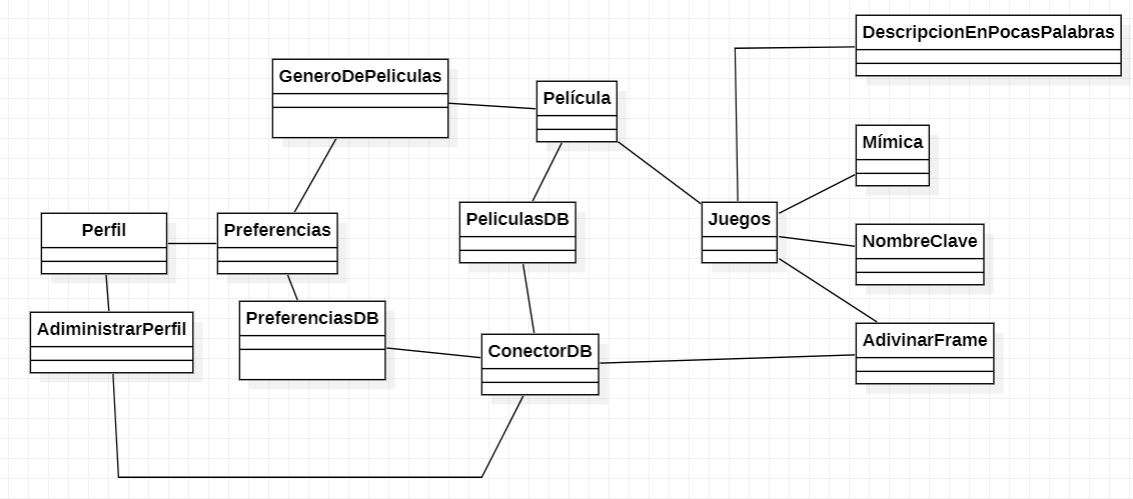
\includegraphics[width=1.2\textwidth]{DiagramaDeClasesFriendsNight.png}

	\caption{Diagrama de clases}
	\label{DiagramaClases}
\end{center}
\vspace{1cm}
%nota mental: puedo poner espacios con \bigskip o con \vspace{1cm} ...  \bigskip es irónicamente más pequeño
%%%%%%%%%%%%%%%%%%%%%%%%%%%%%%
\section{Diagramas de Secuencia:}
\fontsize{14}{18}\selectfont
\par 
A continuación van los diagramas de secuencia para los distintos casos de uso.

El primero refiere al caso de buscar un juego:

\begin{center}
	\centering
		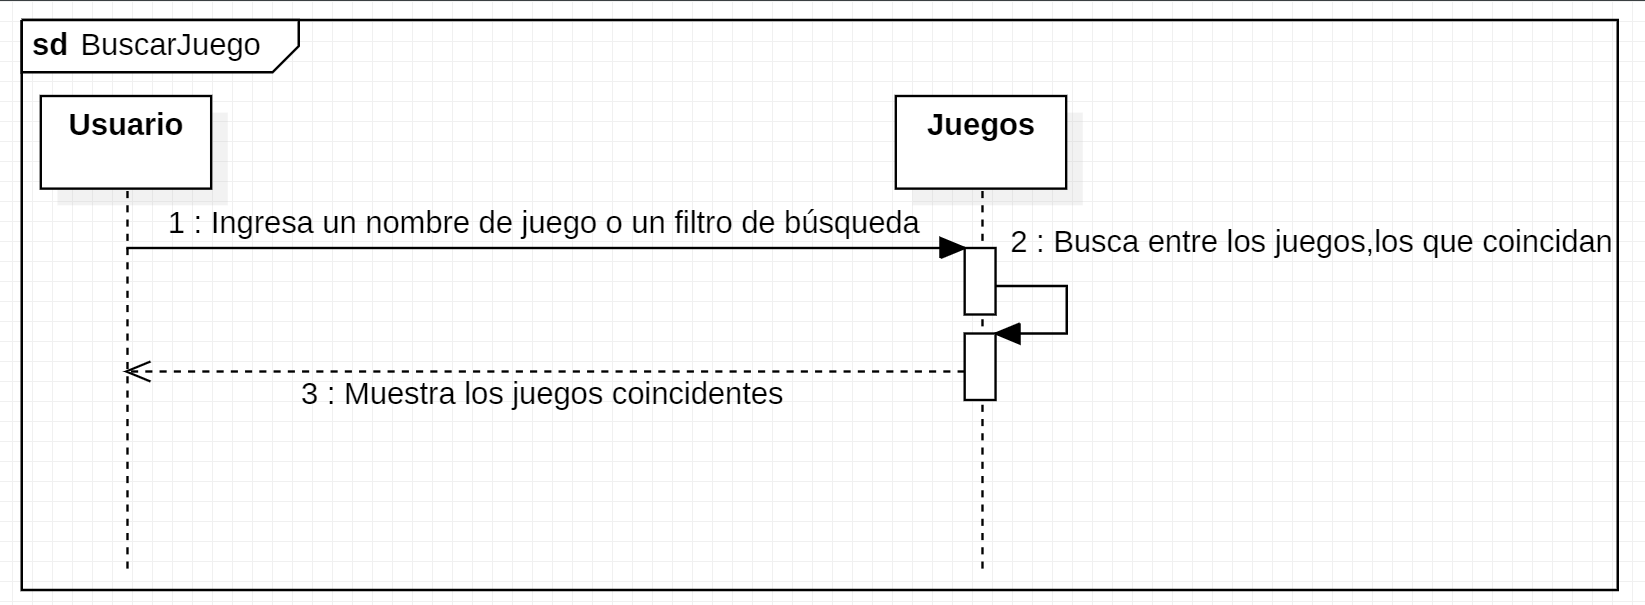
\includegraphics[width=1.2\textwidth]{DSFNBuscarJuego.png}

	\caption{Diagrama de secuencia para buscar un juego}
	\label{DSFNBuscarJuego}
\end{center}

\begin{center}
	\centering
		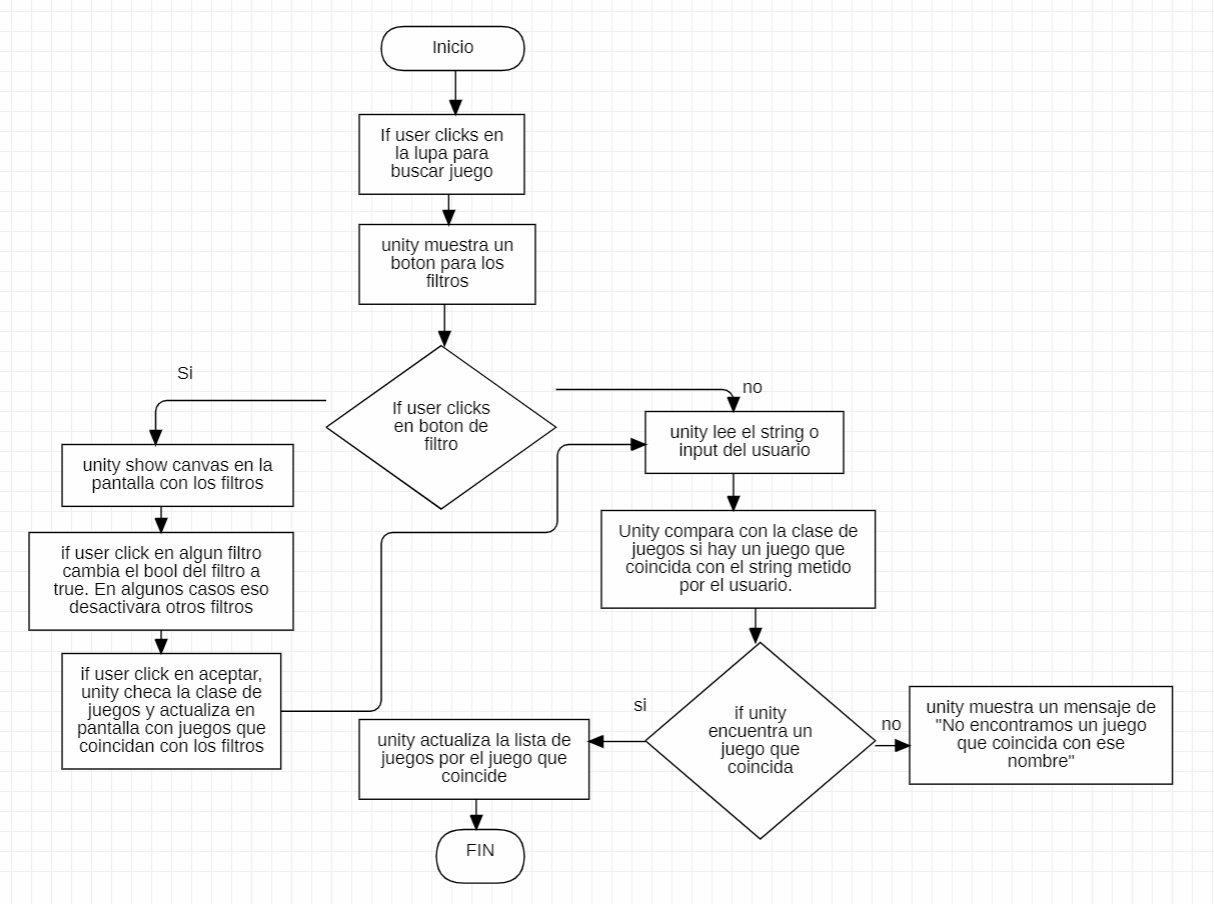
\includegraphics[width=1.2\textwidth]{DFFNBuscarJuego.png}

	\caption{Diagrama de flujo para buscar un juego}
	\label{DFFNBuscarJuego}
\end{center}
%%%%%%%%%%%%%%%%%%%%%
\bigskip
\fontsize{14}{18}\selectfont
\par 
En el segundo diagrama se plasma como sería la creación y edición de un nuevo perfil:

\begin{figure}[h]
    \begin{flushleft}
        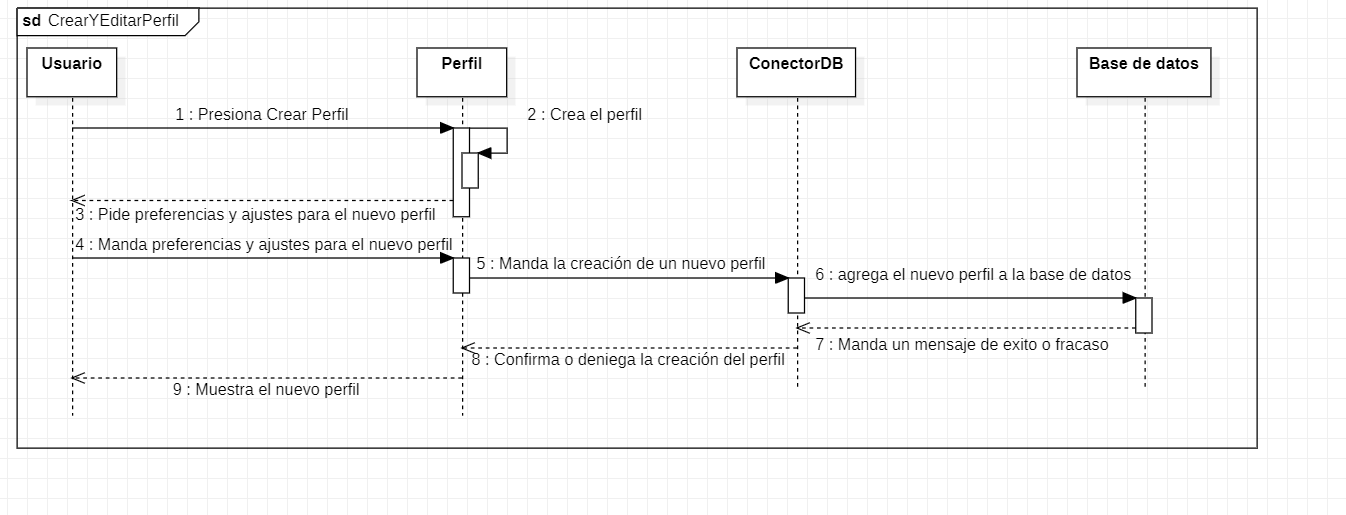
\includegraphics[width=1.2\textwidth]{DSFNCrearYEditarPerfil.png}
        \caption{Diagrama de secuencia para crear y editar un perfil nuevo}
        \label{DSFNCrearYEditarPerfil}
    \end{flushleft}
\end{figure}


\begin{center}
	\centering
		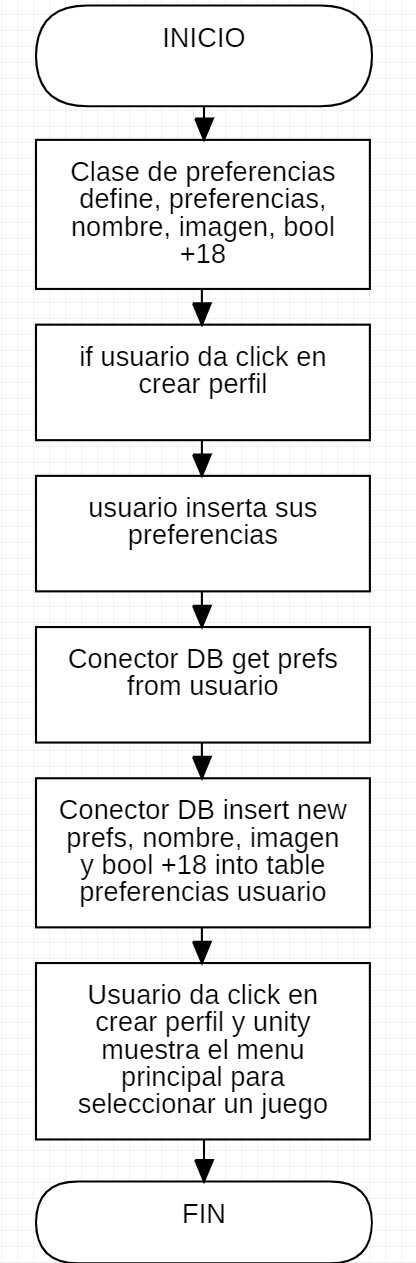
\includegraphics[width=0.5\textwidth]{DFFNCrearYEditarPerfil.png}

	\caption{Diagrama de flujo para crear y editar un perfil nuevo}
	\label{DFFNCrearYEditarPerfil}
\end{center}

\bigskip
%%%%%%%%%%%%%%%%%%%%%%%
\fontsize{14}{18}\selectfont
\par 
En el tercer diagrama propone la secuencia para la edición de la información o preferencias de un perfil ya existente:

\begin{figure}[h]
    \begin{flushleft}
        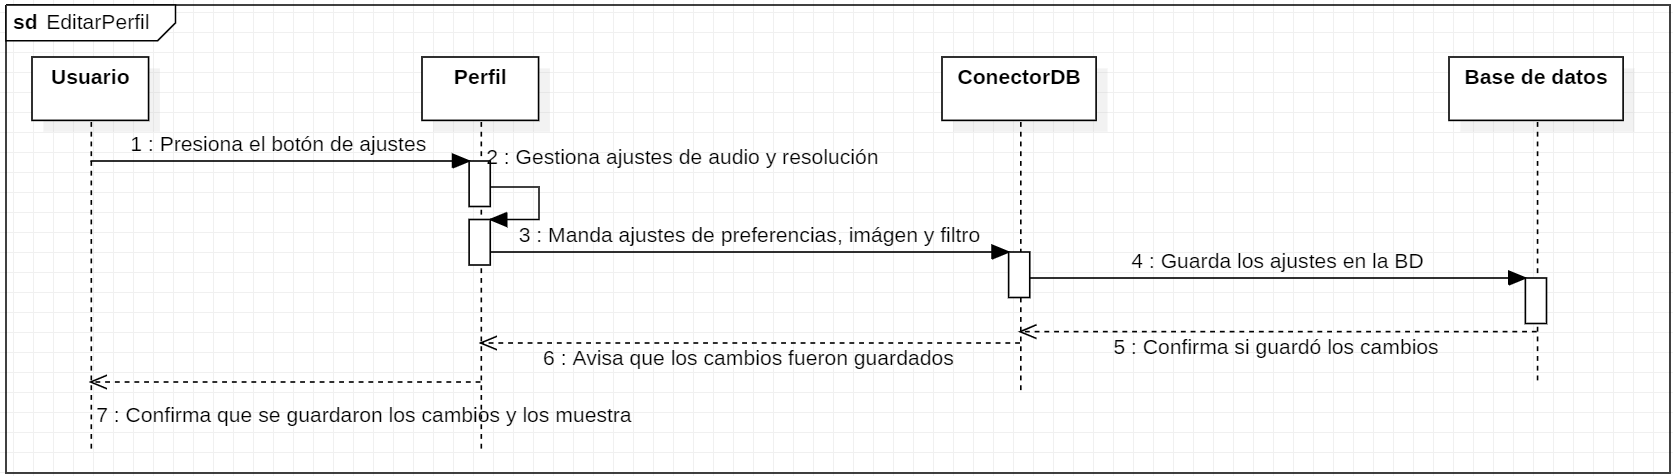
\includegraphics[width=1.2\textwidth]{DSFNEditarPerfil.png}
        \caption{Diagrama de secuencia para editar un perfil ya existente}
        \label{DSFNEditarPerfil}
    \end{flushleft}
\end{figure}


\begin{center}
	\centering
		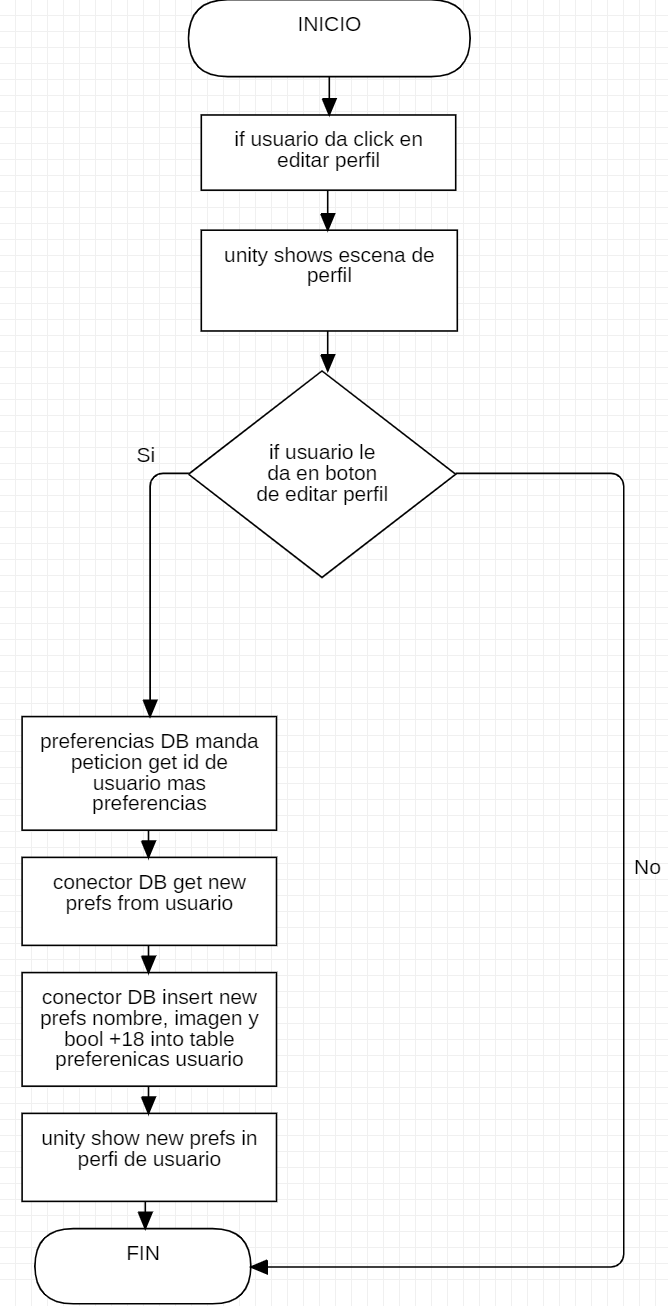
\includegraphics[width=0.4\textwidth]{DFFNEditarPerfil.png}

	\caption{Diagrama de flujo para editar un perfil ya existente}
	\label{DFFNEditarPerfil}
\end{center}

\bigskip

%%%%%%%%%%%%%%%%%%%%%%%
\fontsize{14}{18}\selectfont
\par 
El cuarto diagrama plantea la elección de un juego, en este caso no se contempla un diagrama de flujo ya que este viene incluido en los diagramas de flujo de cada juego respectivamente, sin embargo, se comtempla su diagrama de secuencia pues es necesario detallar las clases de donde obtiene la información necesaria:

\begin{figure}[h]
    \begin{flushleft}
        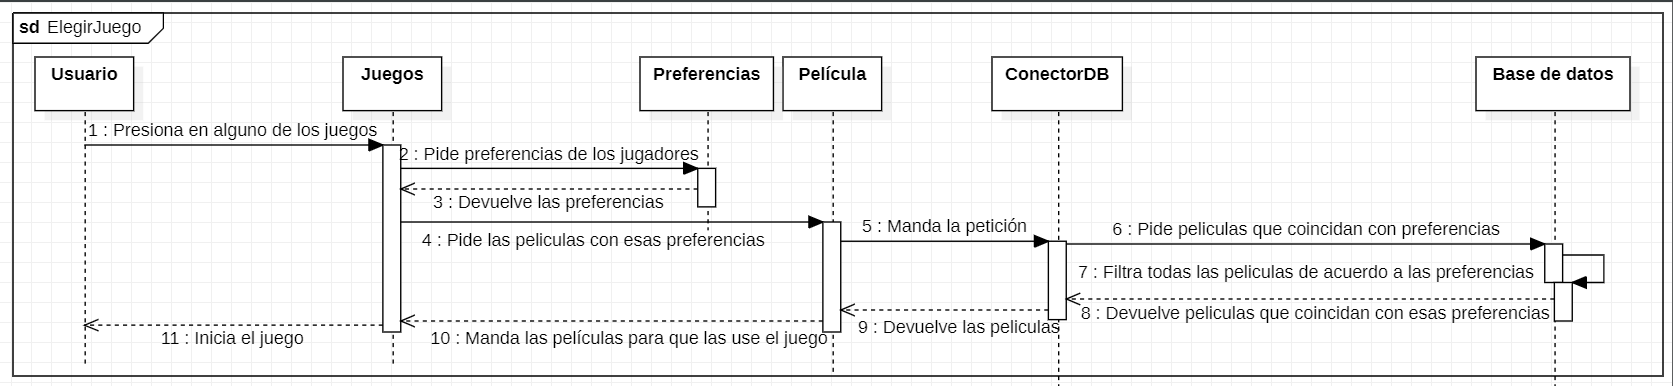
\includegraphics[width=1.3\textwidth]{DSFNElegirJuego.png}
        \caption{Diagrama de secuencia para elegir un juego}
        \label{DSFNElegirJuego}
    \end{flushleft}
\end{figure}

\bigskip
%%%%%%%%%%%%%%%%%
\fontsize{14}{18}\selectfont
\par 
El quinto diagrama propone la secuencia para cambiar las opciones de la interfaz de configuración:

\begin{center}
	\centering
		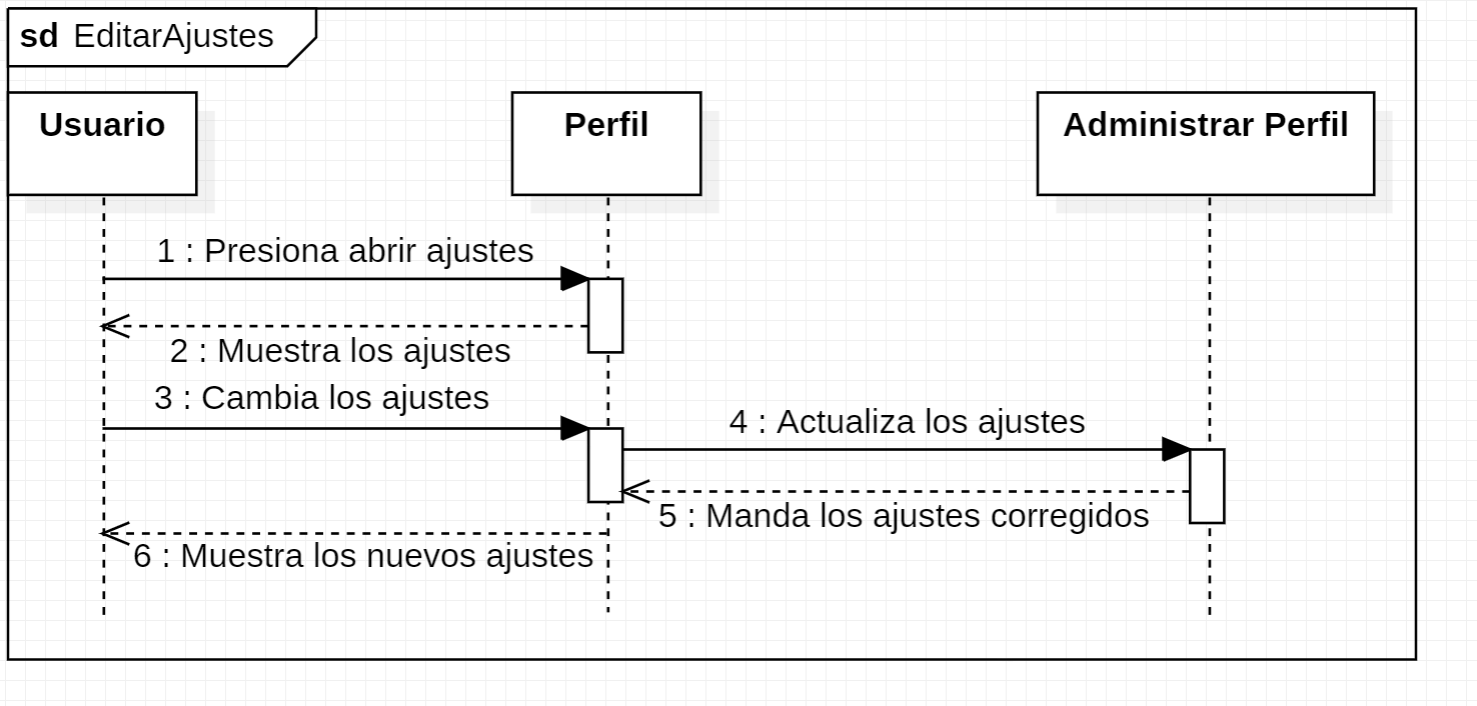
\includegraphics[width=1\textwidth]{DSFNEditarAjustes.png}

	\caption{Diagrama de secuencia para editar las opciones en configuración}
	\label{DSFNopcionesConfig}
\end{center}

\begin{center}
	\centering
		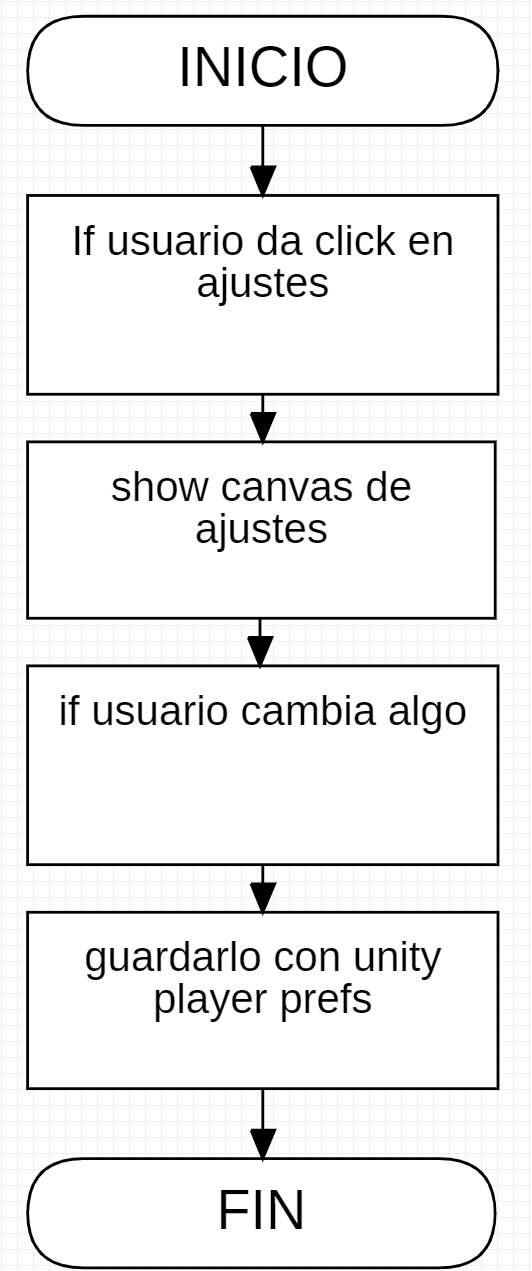
\includegraphics[width=0.4\textwidth]{DFFNEditarAjustes.png}

	\caption{Diagrama de flujo para editar las opciones en configuración}
	\label{DFFNopcionesConfig}
\end{center}

\bigskip
%%%%%%%%%%%%%%%%%%%%%%
\fontsize{14}{18}\selectfont
\par 
En el sexto diagrama se propone la secuencia para regresar al menu principal:

\begin{center}
	\centering
		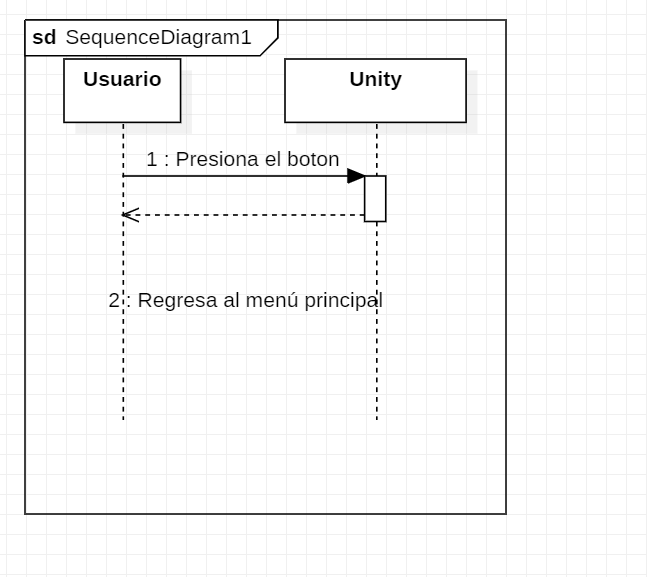
\includegraphics[width=0.9\textwidth]{DSFNRegresarAMenu.png}

	\caption{Diagrama de secuencia para regresar al menu principal}
	\label{DSFNRegresarAMenu}
\end{center}


\begin{center}
	\centering
		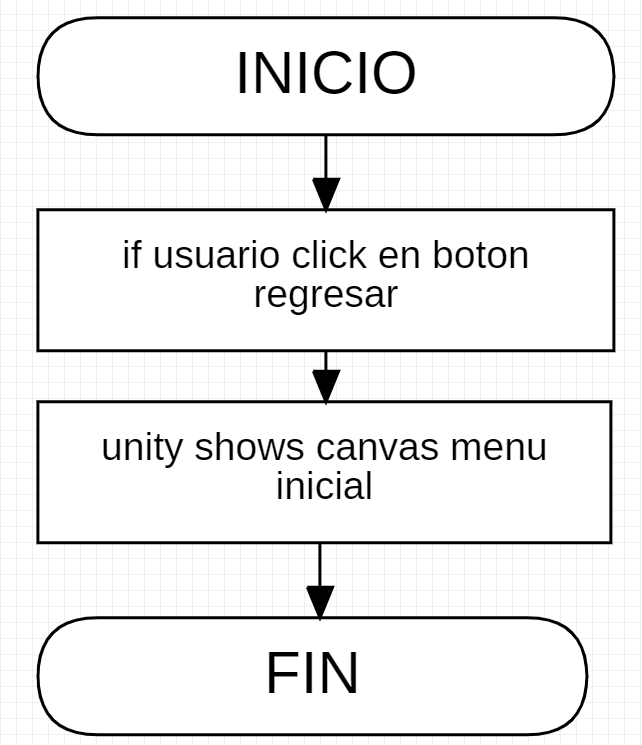
\includegraphics[width=0.4\textwidth]{DFFNRegresarAMenu.png}

	\caption{Diagrama de flujo para regresar al menu principal}
	\label{DFFNRegresarAMenu}
\end{center}


\bigskip
%%%%%%%%%%%%%%%55
\fontsize{14}{18}\selectfont
\par 
Para el septimo diagrama plantea el contacto a soporte, sin embargo, esta opción dependera del tiempo de desarrollo de la aplicación:

\begin{figure}[h]
    \begin{flushleft}
        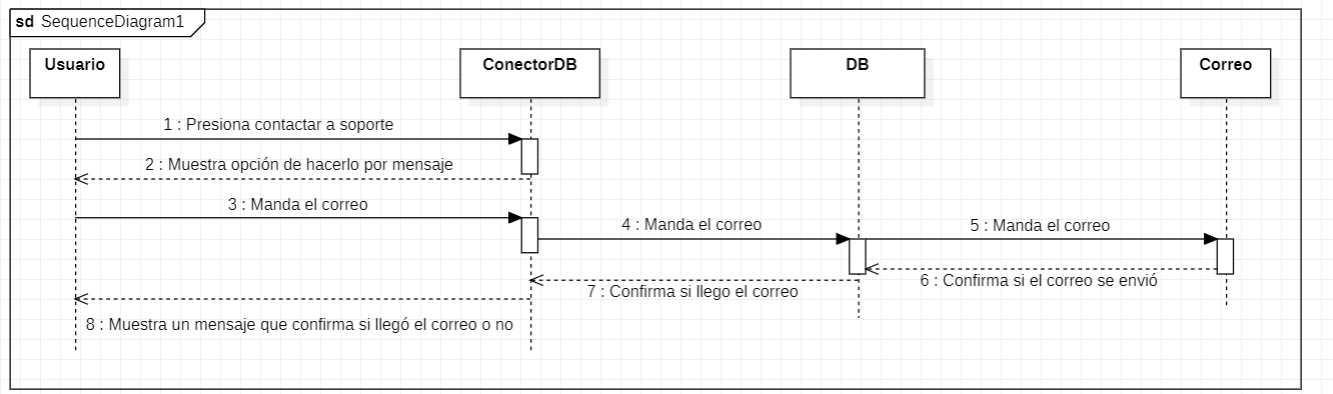
\includegraphics[width=1.3\textwidth]{DSFNContactarSoporte.png}
        \caption{Diagrama de secuencia para contactar a soporte}
        \label{DSFNContactoSoporte}
    \end{flushleft}
\end{figure}


	\centering
		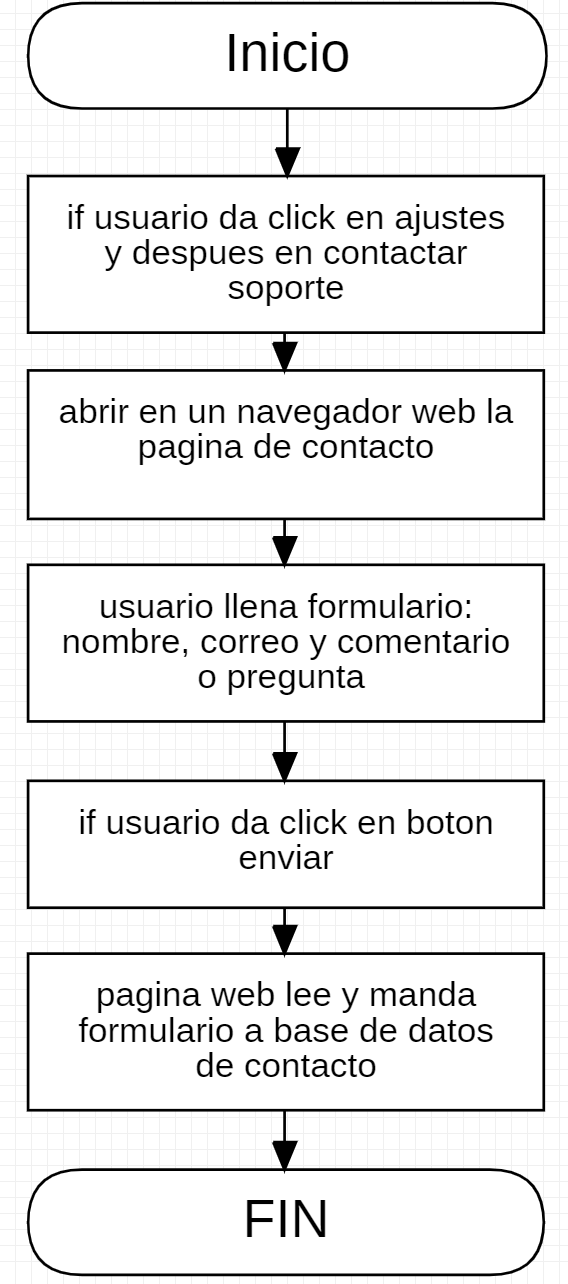
\includegraphics[width=0.5\textwidth]{DFFNContactarSoporte.png}

	\caption{Diagrama de flujo para contactar a soporte}
	\label{DFFNContactoSoporte}
\end{center}


%%%%%%%%%%%%%%%%
\bigskip
\fontsize{14}{18}\selectfont
\par 
En el octavo diagrama se propone la secuencia para jugar el juego de Adivina Frame  y el diagrama de flujo respectivo:

\begin{center}
	\centering
		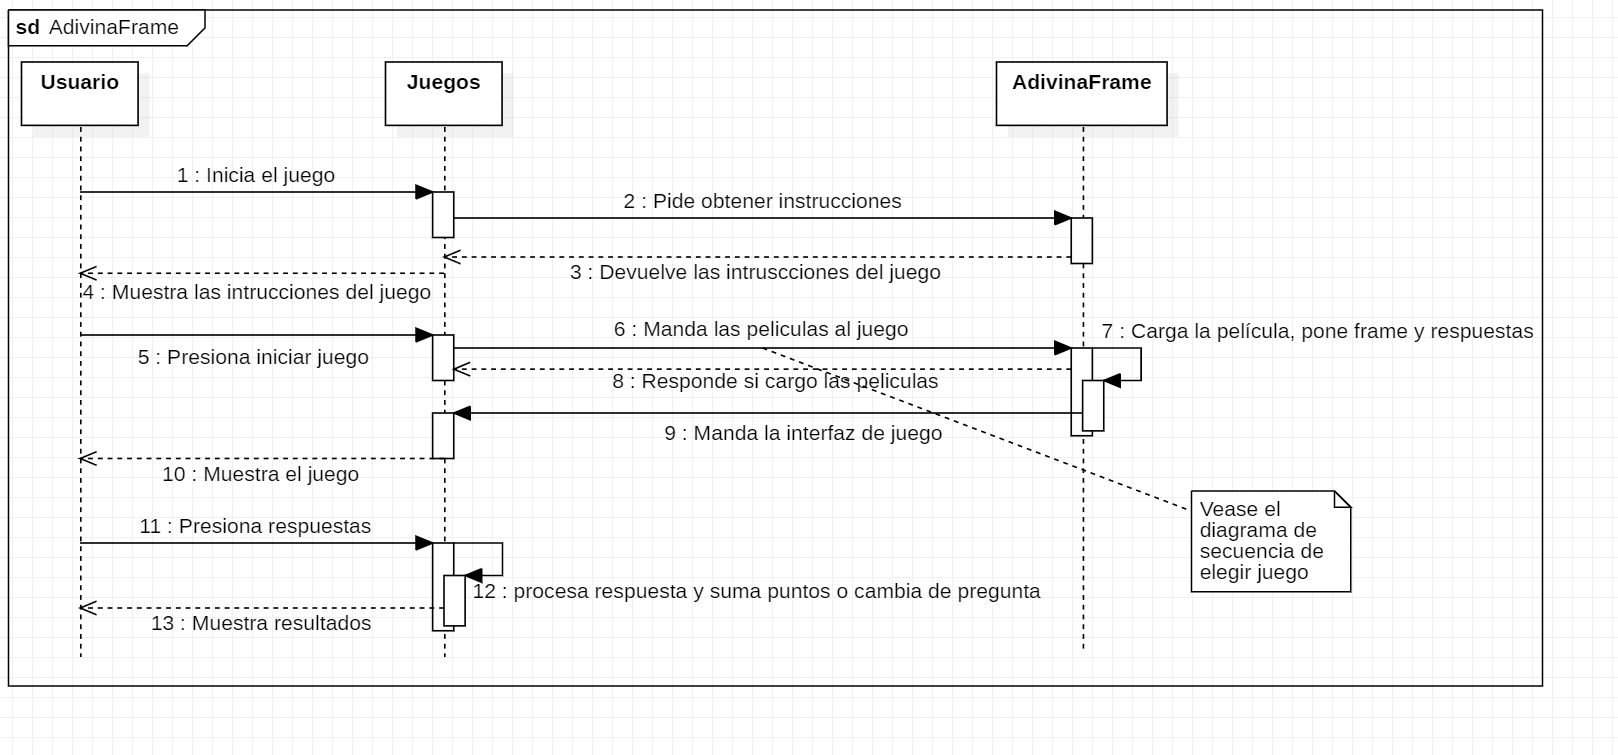
\includegraphics[width=1.3\textwidth]{DSFNAdvinaFrame.png}

	\caption{Diagrama de secuencia para jugar Adivina Frame}
	\label{DSFNAdivinaFrame}
\end{center}

\begin{center}
	\centering
		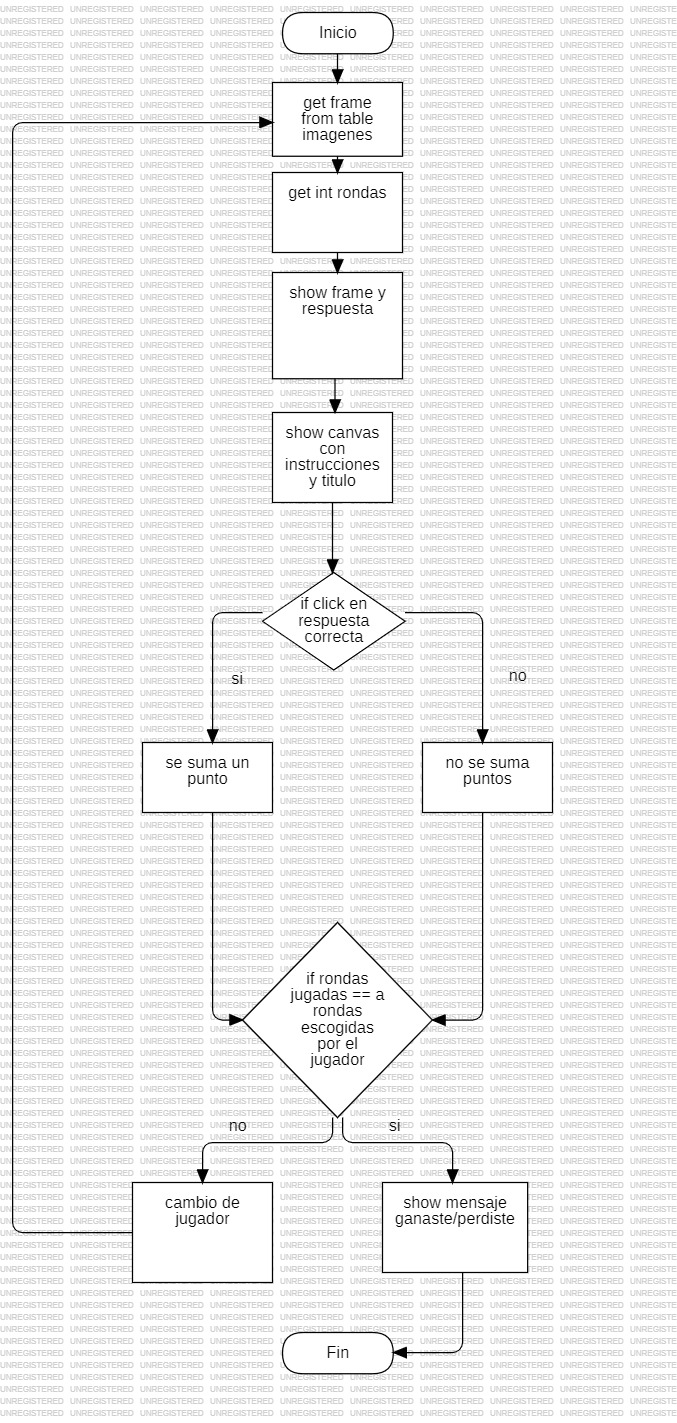
\includegraphics[width=0.7\textwidth]{DFFNAdvinaFrame.png}

	\caption{Diagrama de flujo para jugar Adivina Frame}
	\label{DFFNAdivinaFrame}
\end{center}
%%%%%%%%%%%%%%%%%%%%%%%%5
\bigskip
\fontsize{14}{18}\selectfont
\par 
En el noveno diagrama se propone la secuencia para jugar el juego de descripción en pocas palabras  y el diagrama de flujo respectivo:

\begin{center}
	\centering
		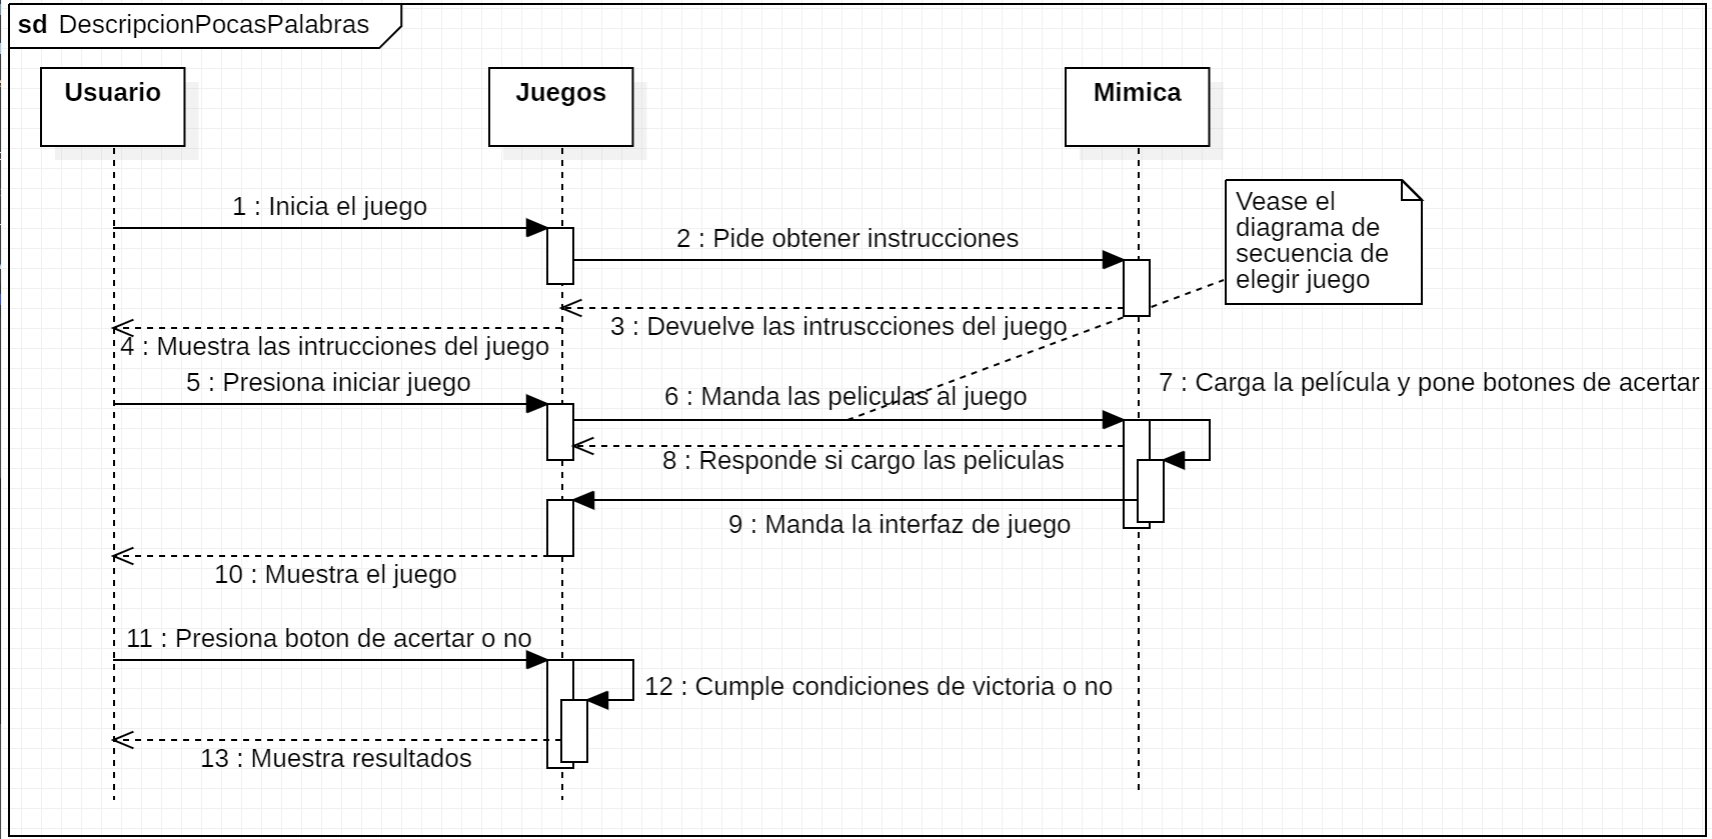
\includegraphics[width=1.29\textwidth]{DSFNDescripcionEnPocasPalabras.png}

	\caption{Diagrama de secuencia para jugar descripción en pocas palabras}
	\label{DSFNDescric}
\end{center}
\begin{center}
	\centering
		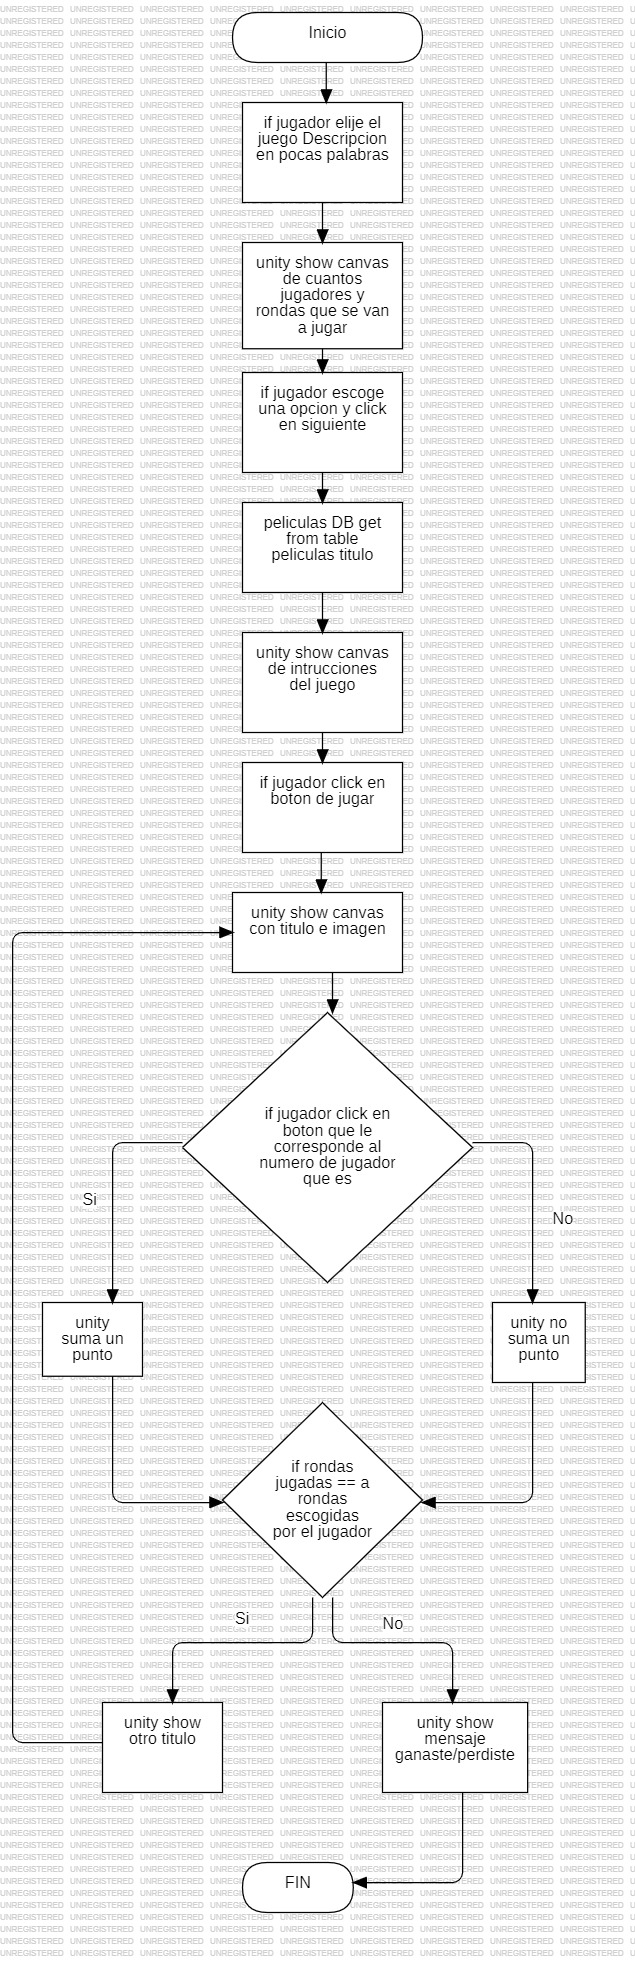
\includegraphics[width=0.56\textwidth]{DFFNDescripcionEnPocasPalabras.jpg}

	\caption{Diagrama de flujo para jugar descripción en pocas palabras}
	\label{DFFNDescr}
\end{center}
%%%%%%%%%%%%%%%%%%%5
\bigskip
\fontsize{14}{18}\selectfont
\par 
En el decimo diagrama se propone la secuencia para jugar el juego de mímica y el diagrama de flujo respectivo:

\begin{center}
	\centering
		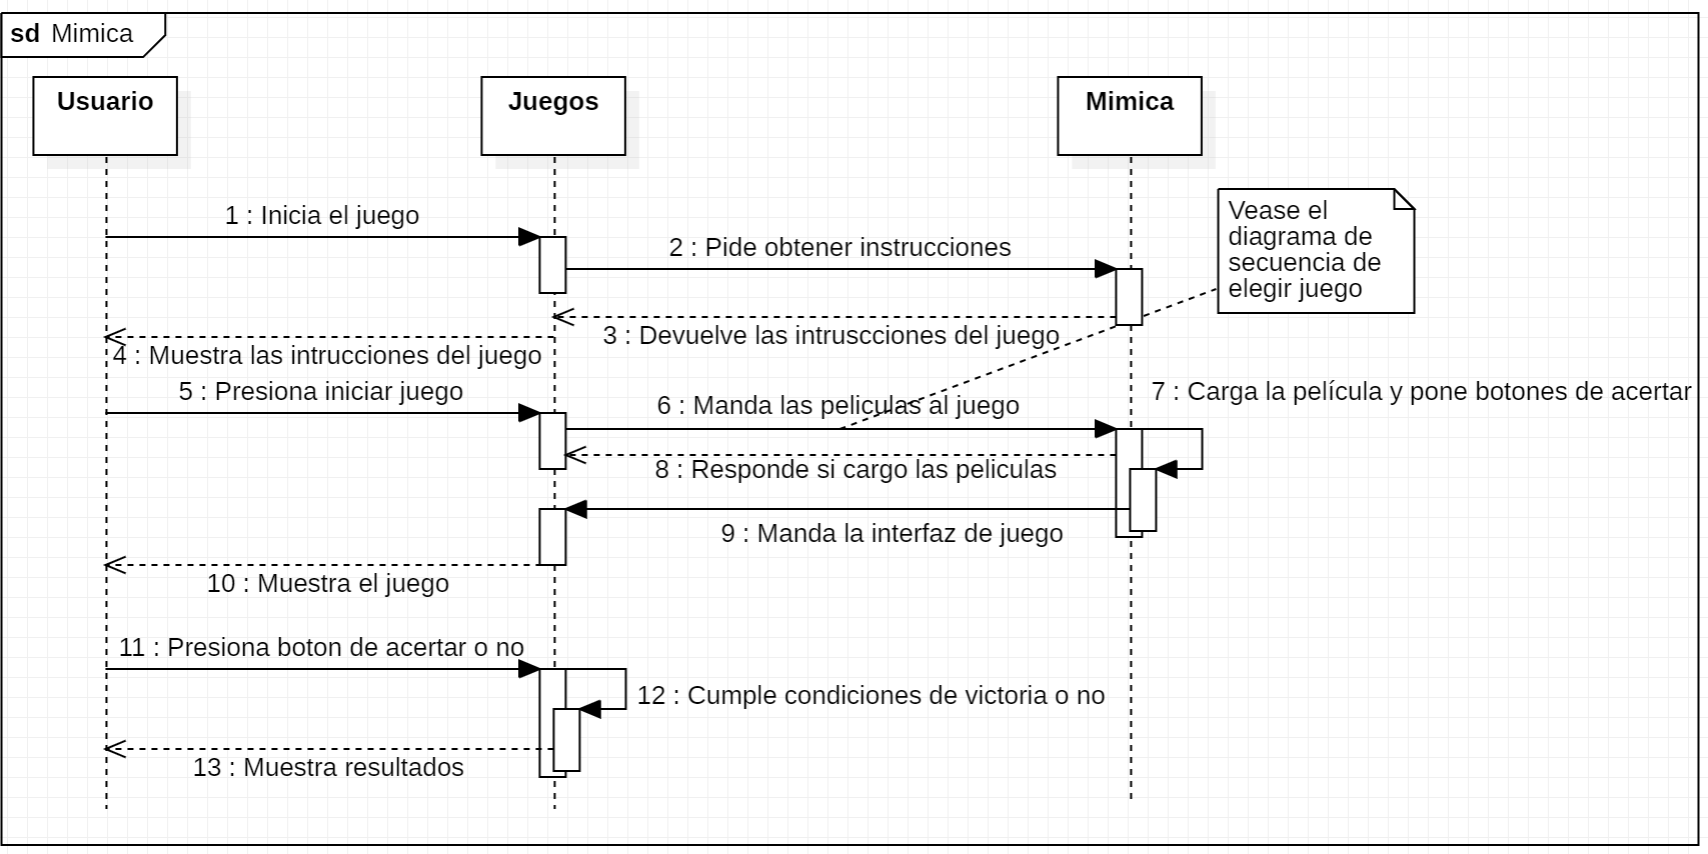
\includegraphics[width=1.29\textwidth]{DSFNMimica.png}

	\caption{Diagrama de secuencia para jugar Mímica}
	\label{DSFNMimica}
\end{center}

\begin{center}
	\centering
		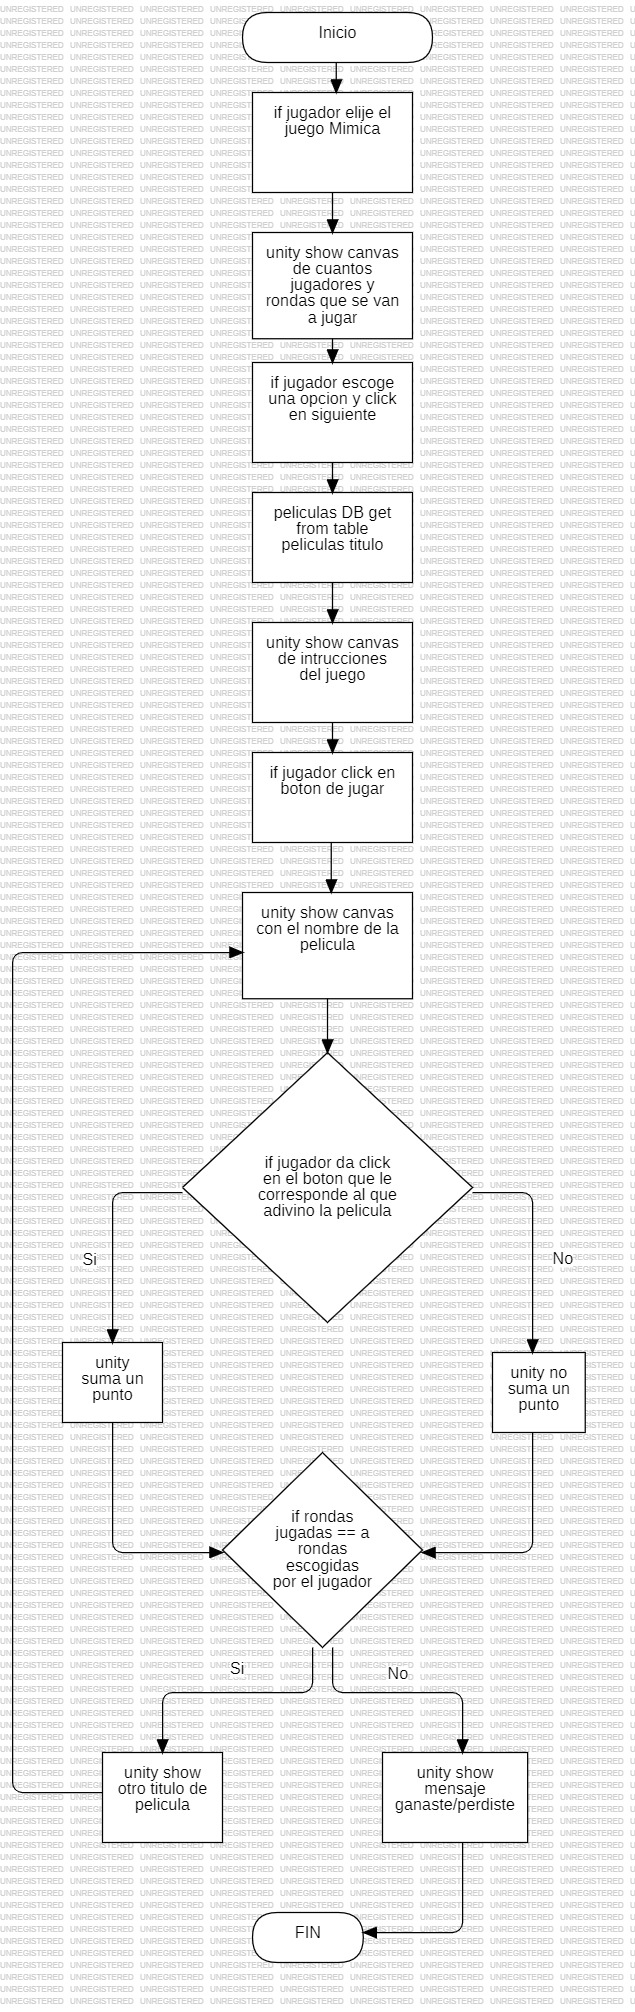
\includegraphics[width=0.5\textwidth]{DFFNMimica.jpg}

	\caption{Diagrama de flujo para jugar Mímica}
	\label{DFFNMimica}
\end{center}
%%%%%%%%%%%%%%%%%%%5
\bigskip
\fontsize{14}{18}\selectfont
\par 
En el onceavo diagrama se propone la secuencia para jugar el juego de Nombre Clave y el diagrama de flujo respectivo:

\begin{center}
	\centering
		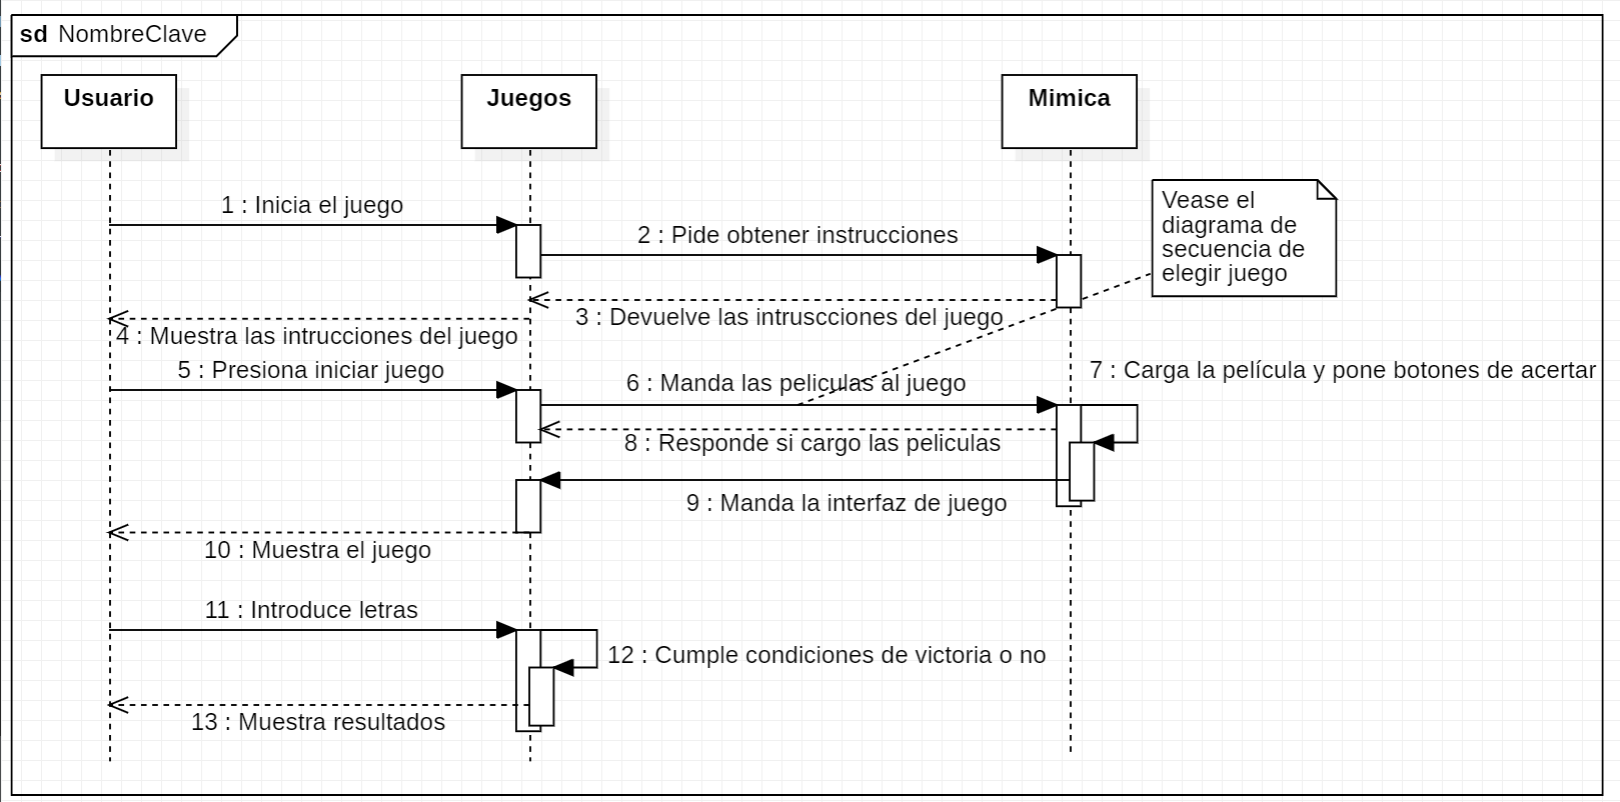
\includegraphics[width=1.29\textwidth]{DSFNNombreClave.png}

	\caption{Diagrama de secuencia para jugar Nombre Clave}
	\label{DSFNC}
\end{center}

\begin{center}
	\centering
		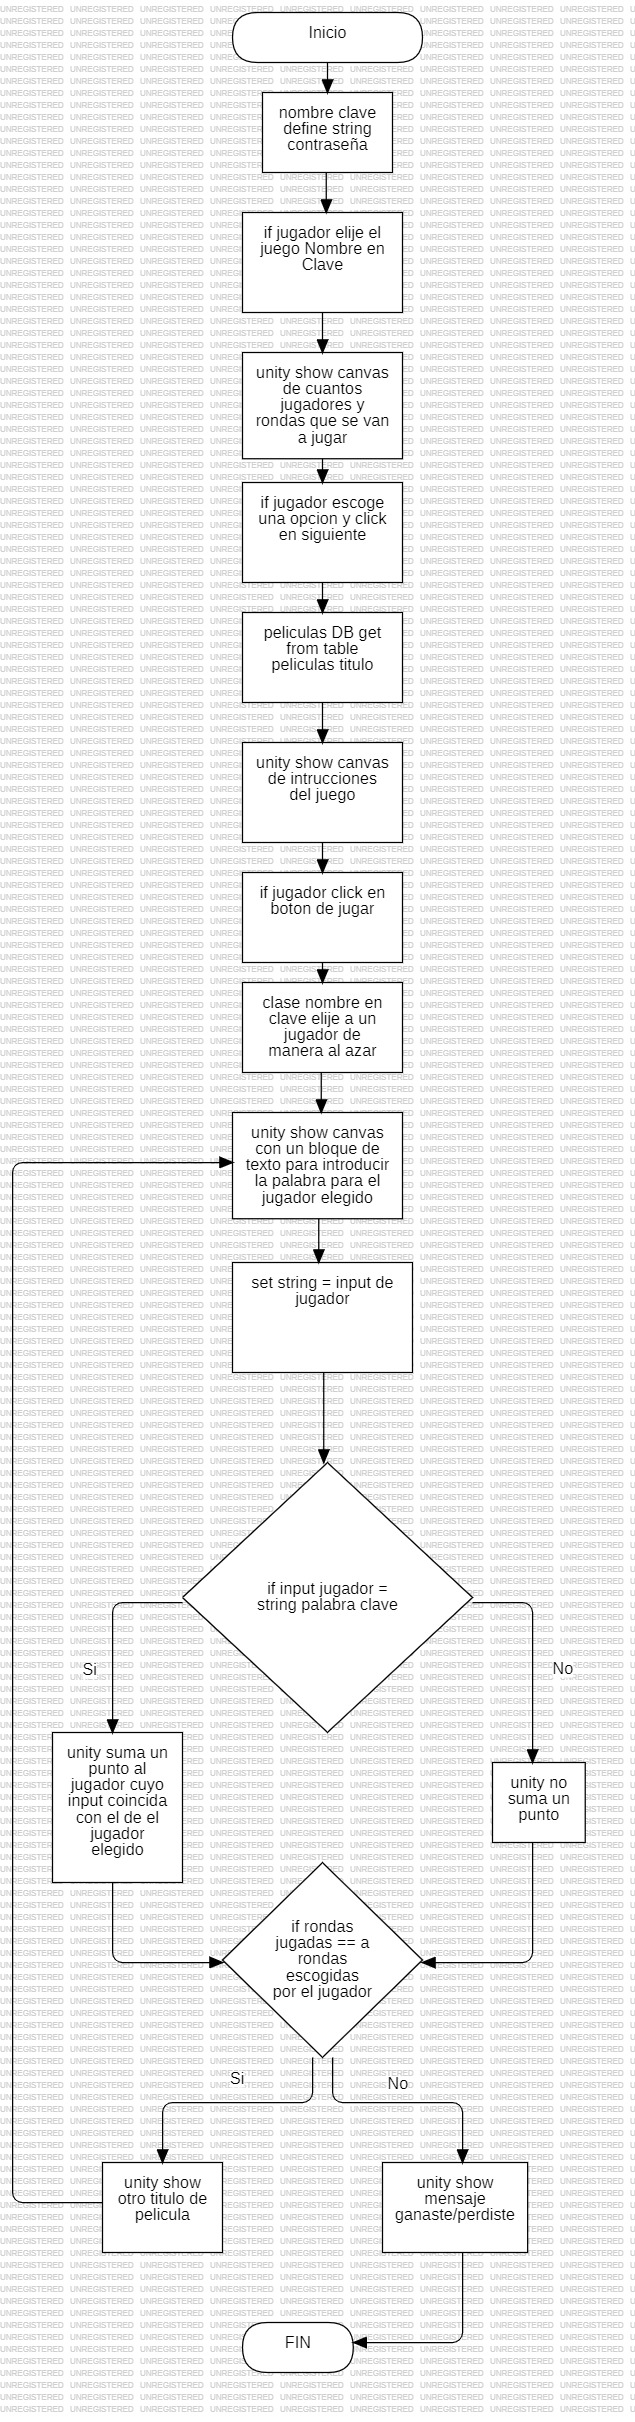
\includegraphics[width=0.4\textwidth]{DFFNNombreEnClave.jpg}

	\caption{Diagrama de flujo para jugar Nombre Clave}
	\label{DSFNC}
\end{center}


%%%%%%%%%%%%%%%%%%%5
\bigskip
\fontsize{14}{18}\selectfont
\par 
En el doceavo diagrama se propone la secuencia para elegir el perfil al iniciar el juego con su diagrama de flujo respectivo:

\begin{figure}[h]
    \begin{flushleft}
        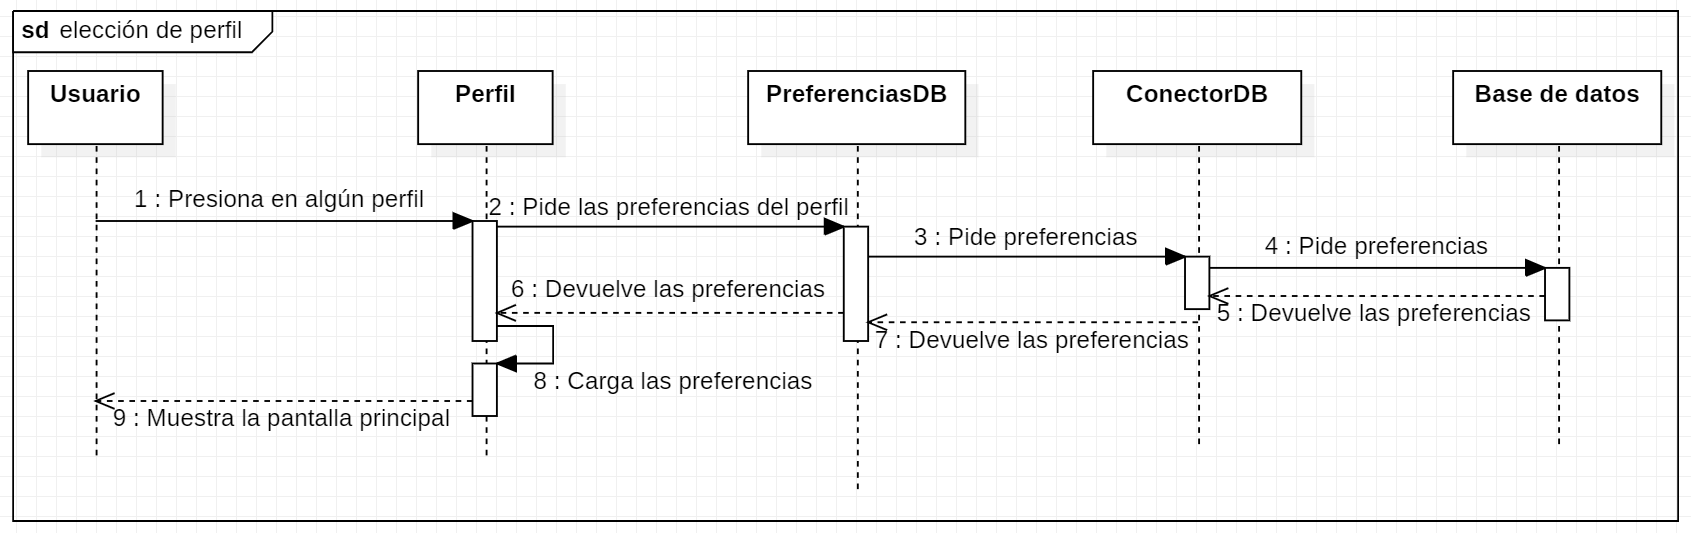
\includegraphics[width=1.3\textwidth]{DSFNElegirPerfil.png}
        \caption{Diagrama de secuencia para elegir perfil}
        \label{DSFNC}
    \end{flushleft}
\end{figure}


\begin{center}
	\centering
		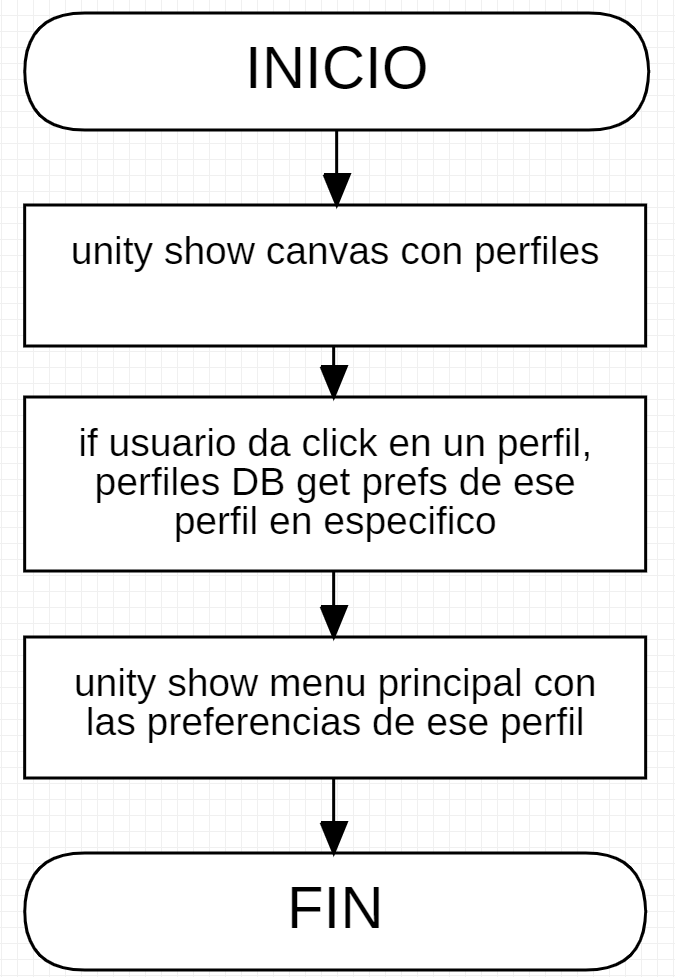
\includegraphics[width=0.3\textwidth]{DFFNElegirPerfil.png}

	\caption{Diagrama de flujo para elegir el perfil}
	\label{DSFNC}
\end{center}
\bigskip
%%%%%%%%%%%%Diagrama de estados%%%%%%%%%%%%%%%%
\section{Diagramas de estados}
\par 
Tenemos dos diagramas de estados, el primer corresponde a los estados al estar en el menu, inmediatamente despues de haber seleccionado un perfil: 

\begin{figure}[h]
    \begin{flushleft}
        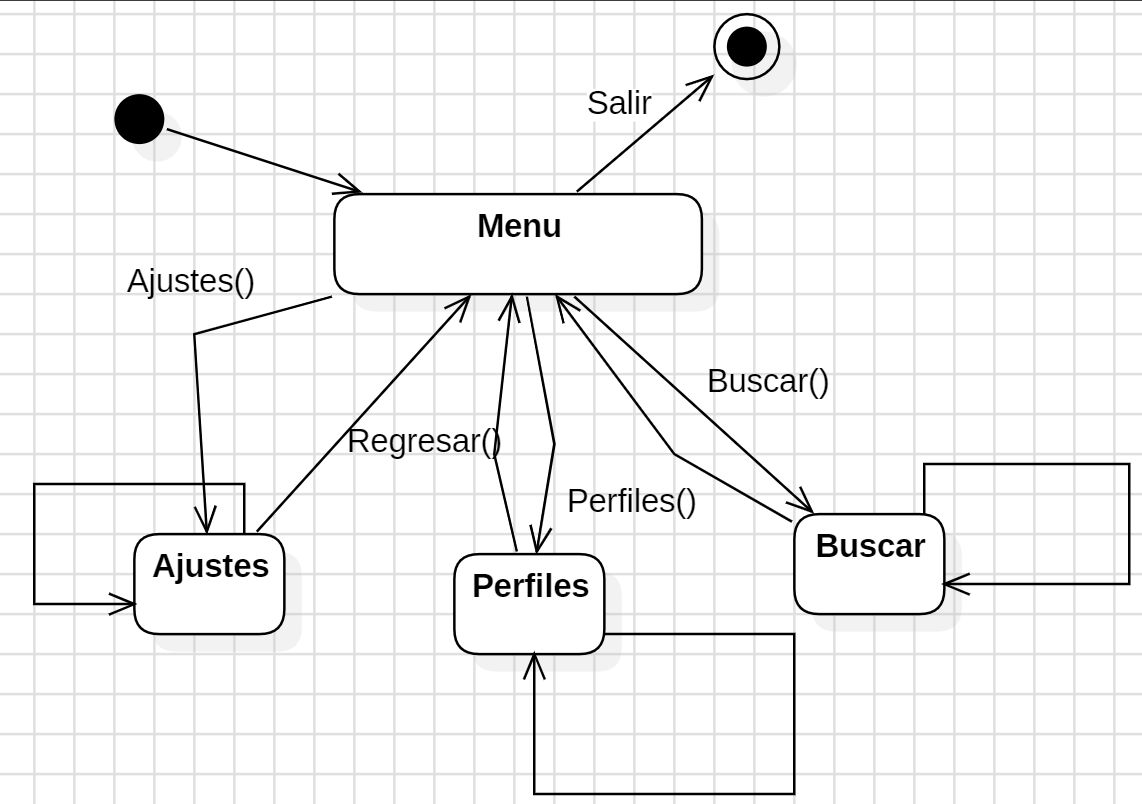
\includegraphics[width=1.3\textwidth]{DiagramaEstadosMenuFN.jpeg}
        \caption{Diagrama de estados del menu}
        \label{DEMFN}
    \end{flushleft}
\end{figure}

\par 
En el diagrama siguiente se muestran los estados del juego al crear un perfil en el juego:  

\begin{figure}[]
    \begin{flushleft}
        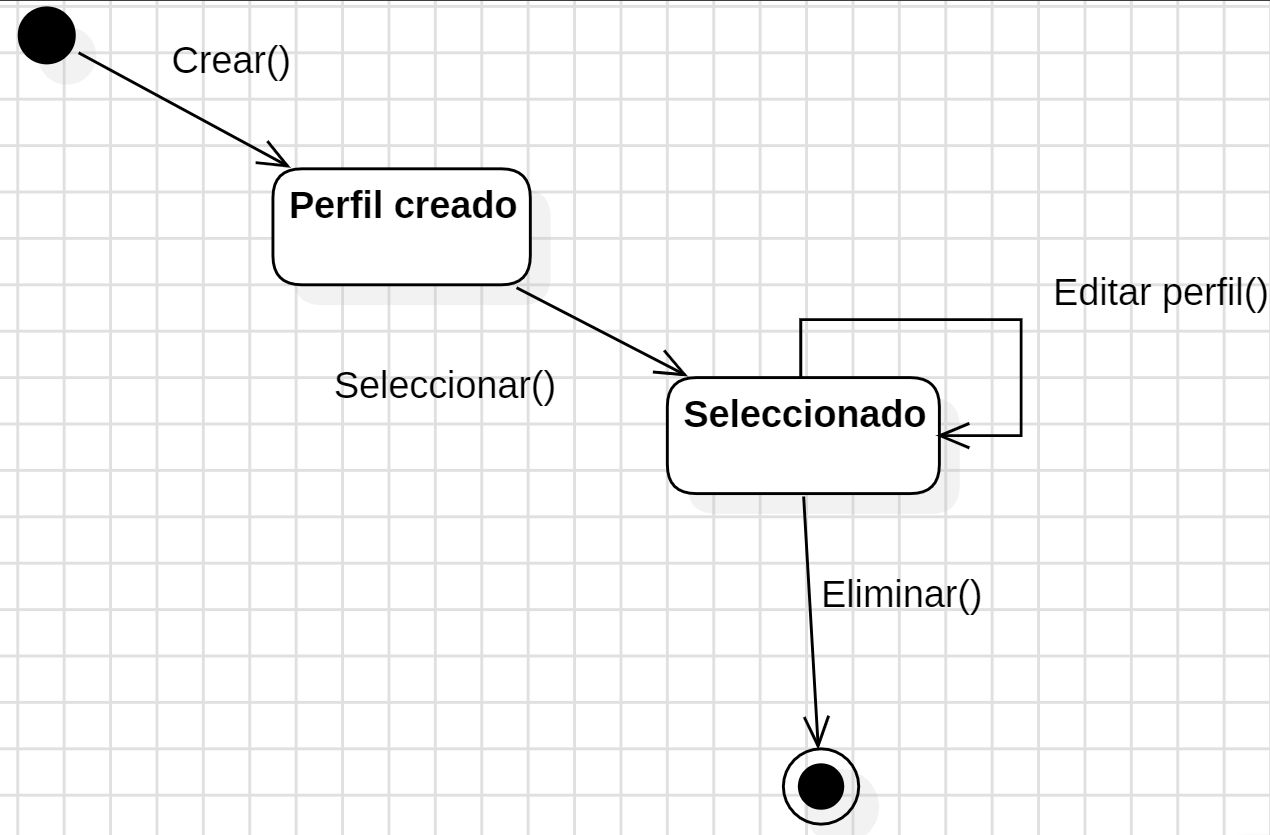
\includegraphics[width=1.2\textwidth]{DiagramaEstadosCrearPerfilFN.jpeg}
        \caption{Diagrama de estados creación de perfil}
        \label{DEFN}
    \end{flushleft}
\end{figure}
\bigskip
%%%%%%%%%%%%%%%%%%MAPA DE SITIO%%%%%%%%%%%%%%%%%%%%
\chapter{Propuesta de pantallas (Mapa de sitio) }
\par 
Para la propuesta de las distintas pantallas se hicieron estos tres bocetos: 
\begin{figure}[h]
		\centering
    \begin{subfigure}{.3\textwidth}
        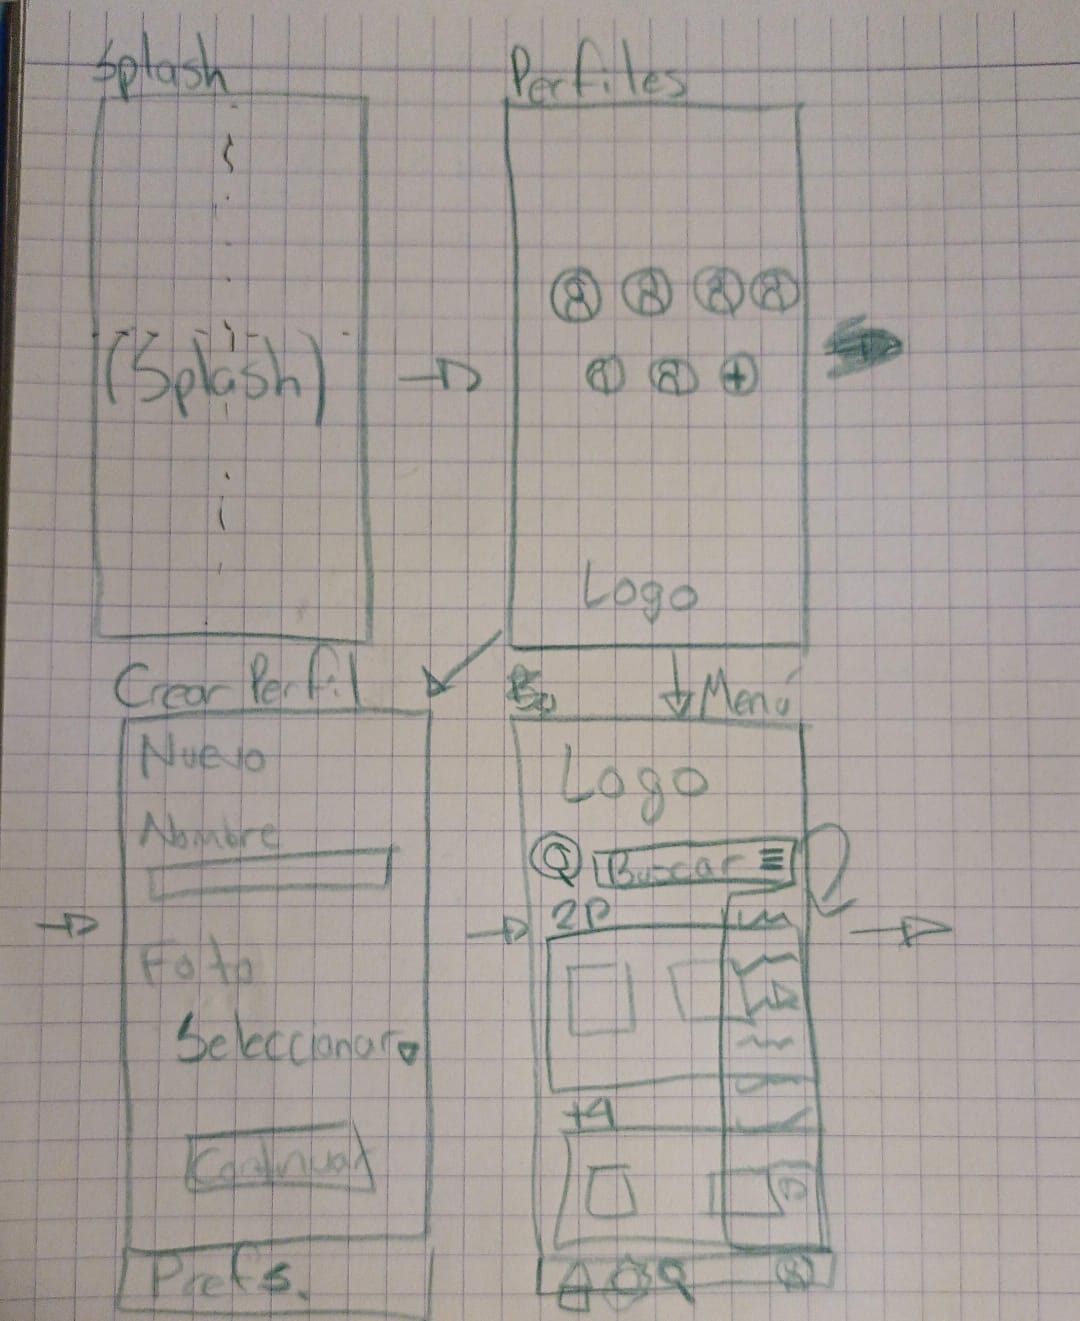
\includegraphics[width=\linewidth]{BocetoInterfacesFN1.jpeg}
        \caption{Bocetos 1 }
        \label{BP1FN}
    \end{subfigure}
		\begin{subfigure}{.3\textwidth}
        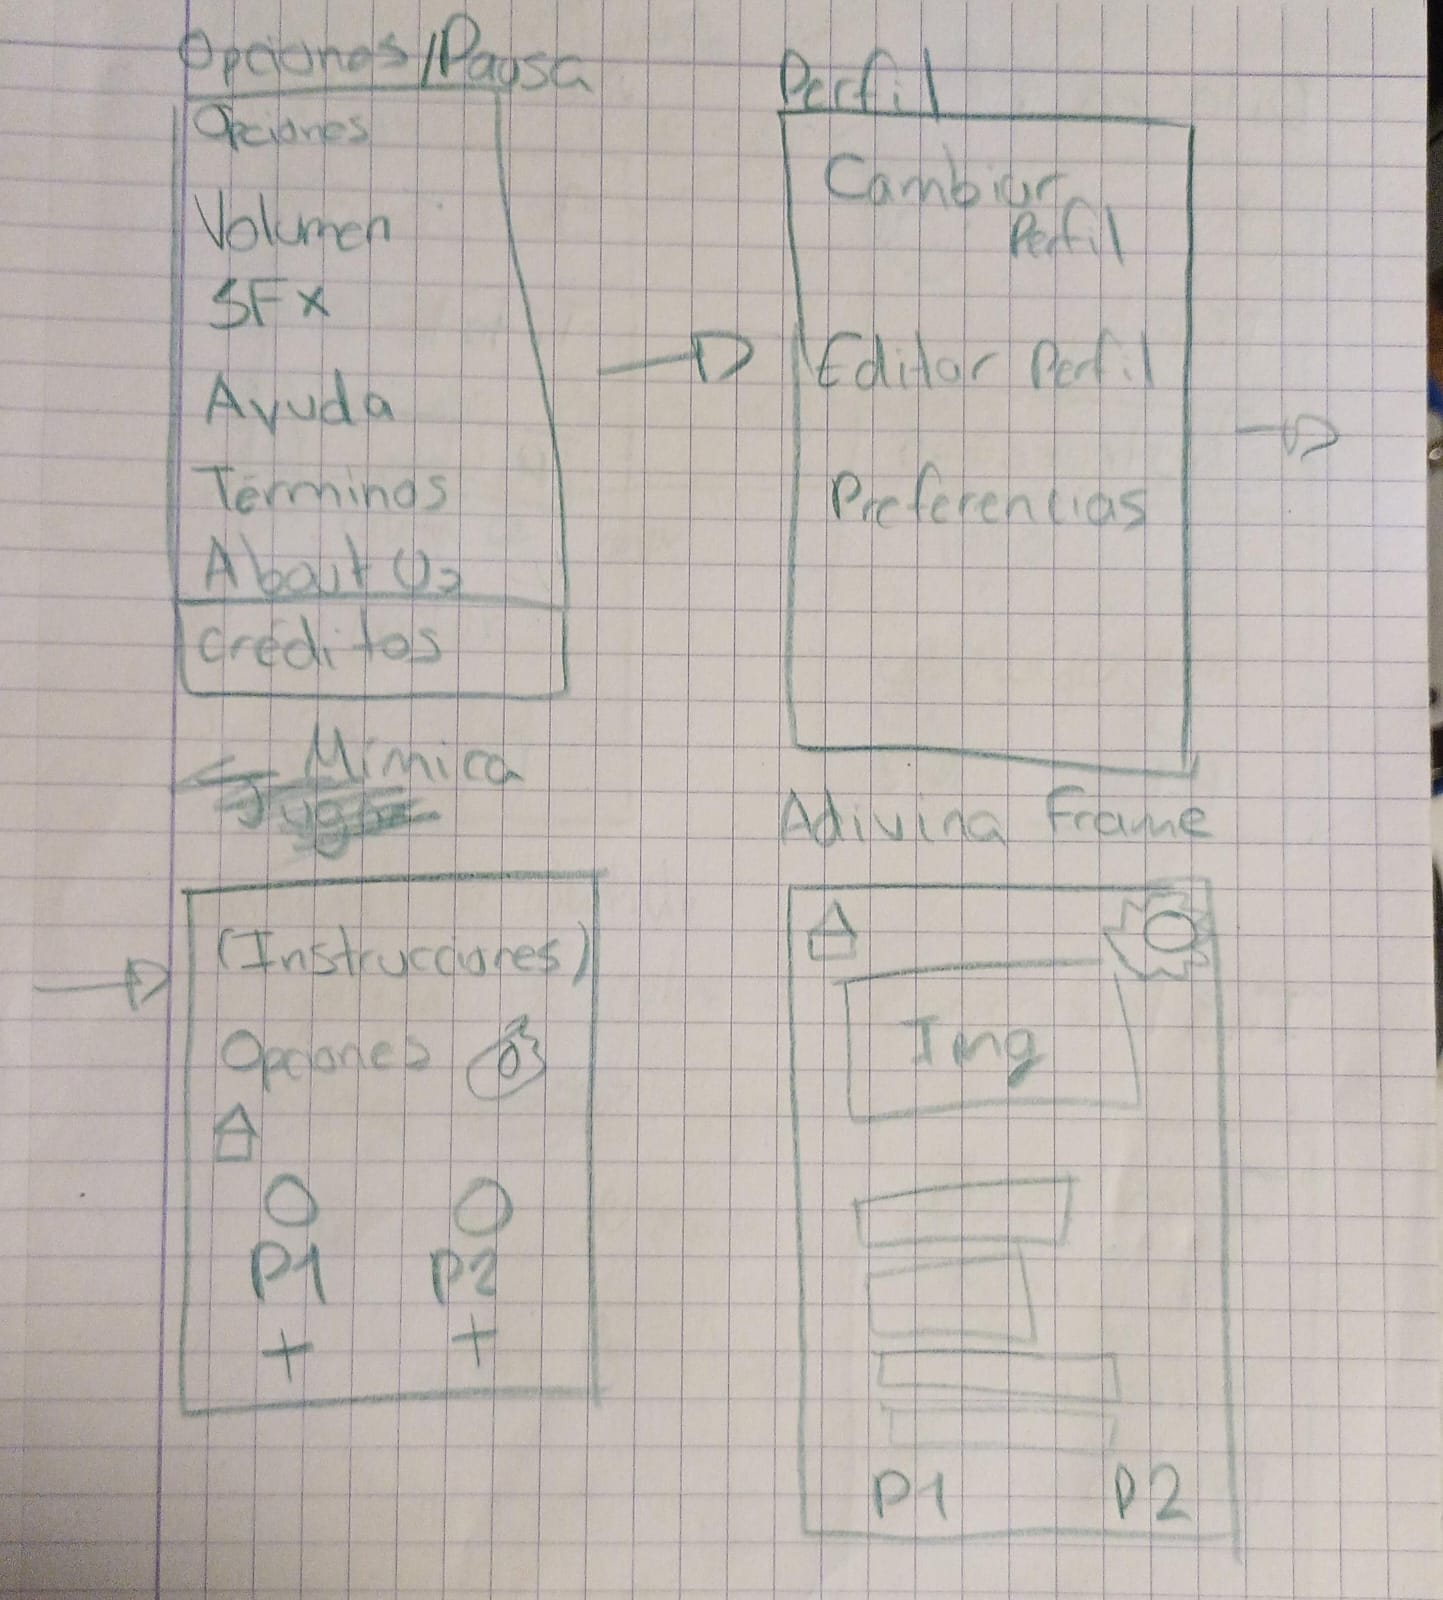
\includegraphics[width=\linewidth]{BocetoInterfacesFN2.jpeg}
        \caption{Boceto 2 }
        \label{BP2FN}
    \end{subfigure}
		\begin{subfigure}{.3\textwidth}
        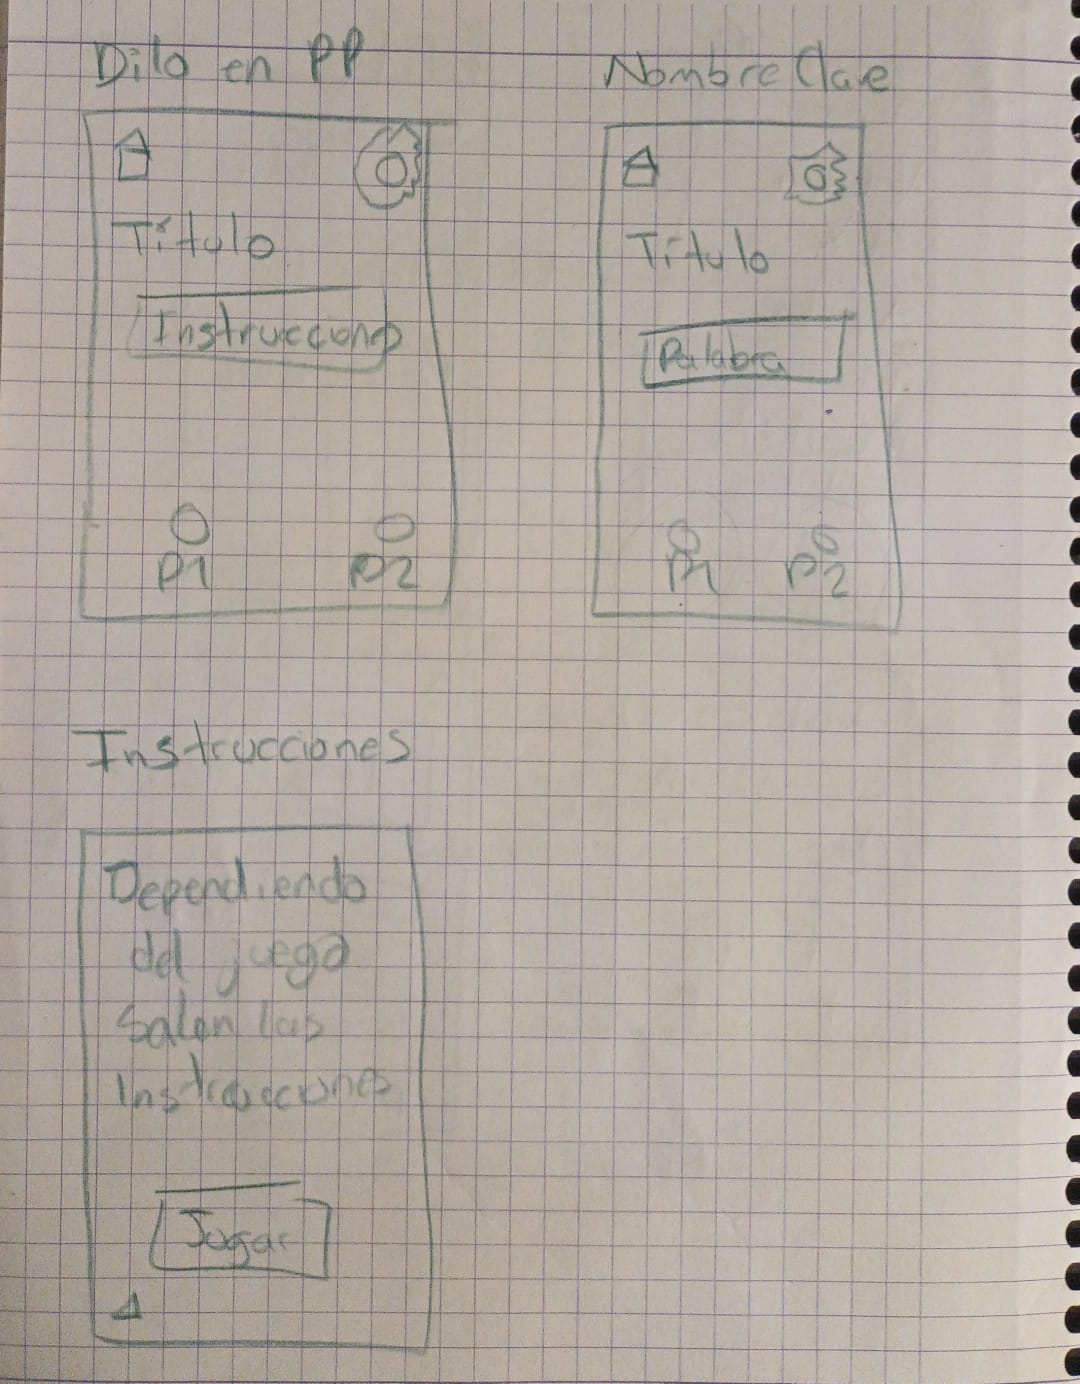
\includegraphics[width=\linewidth]{BocetoInterfacesFN3.jpeg}
        \caption{Boceto 3 }
        \label{BP3FN}
    \end{subfigure}
		\caption{Bocetos de las pantallas}
		\label{BPFN}
\end{figure}
\par Una vez realizado eso, quedo el mapa de sitio con todas las interfaces necesarias: 
\begin{center}
	\centering
		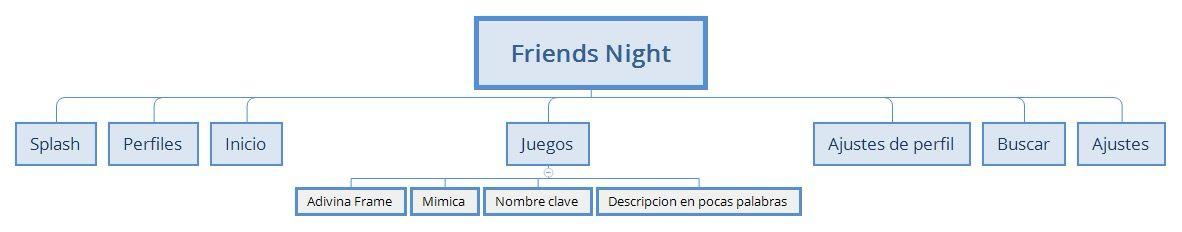
\includegraphics[width=1.2\textwidth]{MapaDeSitioFN.jpeg}

	\caption{Mapa de sitio de Friends Night}
	\label{MSFN}
\end{center}
\vspace{1cm}
%%%%%%%%%%%%%%%%%%%PROTOTIPO EN FIGMA%%%%%%%%%%%
\chapter{Prototipo en Figma}
\p Para tener mas claro la secuencia de como irán las pantallas dentro del juego se realizó un figma del juego para visualizar tanto aspectos gráficos como funcionales: \href{https://www.figma.com/proto/XxxgYRp8yMguil1C3WnmF8/Friend\%C2\%B4s-Night?type=design&node-id=292-2&t=yDlQBRXyiRyzXJ0W-1&scaling=min-zoom&page-id=0\%3A1&starting-point-node-id=255\%3A2&mode=design}{Prototipo en Figma de Friends Night}
\begin{figure}
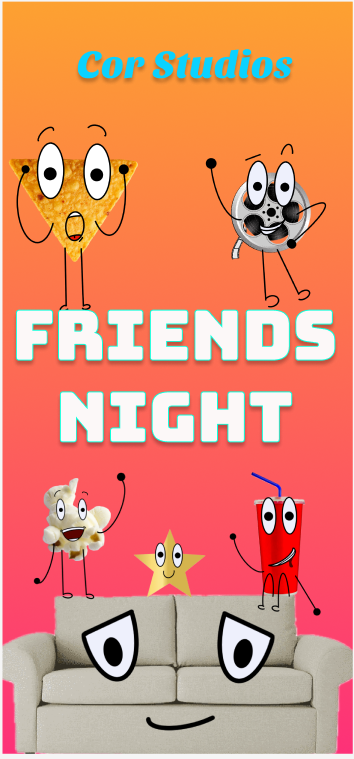
\includegraphics[width=.8\textwidth]{FriendsNightFigma.png}%
\caption{Figma del juego }
\label{Figma}
\end{figure}
%%%%%%%%%%%%%%%%%%%%%%%%%%%%%%%%%%%%%

\part{Identidad}
%%%%%%%%%%%%%%%%%%%%%% IDENTIDAD %%%%%%%%%%%%%%%%%%%%%%%%%%%
\chapter{Identidad}
%%%
\section{Nuestra marca:}
\p El estudio productor del juego que somos nosotros se llama \textbf{\textit{COR Studios}}, y el logo es el siguiente: 
\begin{center}

\includegraphics[width=0.4\textwidth]{logoCOR.png}%
\caption{Logo de COR studios}%
\label{LCS}%
\end{center} 
\p Y surge de que buscamos mostrar pasión por la creación de videojuegos, de ahií que el nombre sea corazón en latín, a su vez, en el logo vemos el símbolo de libertad e innovación que viene implícito por el cohete (Siendo el propio corazón ese cohete)
%%%

\section{Logo del juego}
\begin{figure}[h]

\includegraphics[width=0.7\textwidth]{logofriends.png}%
\caption{Logo del juego Friends Night}%
\label{LFN}%
\end{figure}
\p En este logo podemos ver a palomitas y un refresco, dos elementos asociados al cine, que se reunen a jugar videojuegos, dando la imagen que buscamos de la unión entre videojuegos y el cine, además de la amistad. 

%%%%%
\section{Paleta de color del juego}
\p Para las paletas de color del juego usamos colores asociados al juego mental, sin embargo, para evitar que el color pastel usual de juegos así también brindara una calma que no queremos transmitir, los colores estan saturados o en algunos casos se cambiar por completo la tonalidad. 
En la siguiente imagen se puede ver todas las paletas de color intentadas, pero resalta la cuarta fila pues es la paleta de color principal que estamos usando 
\begin{figure}[h]
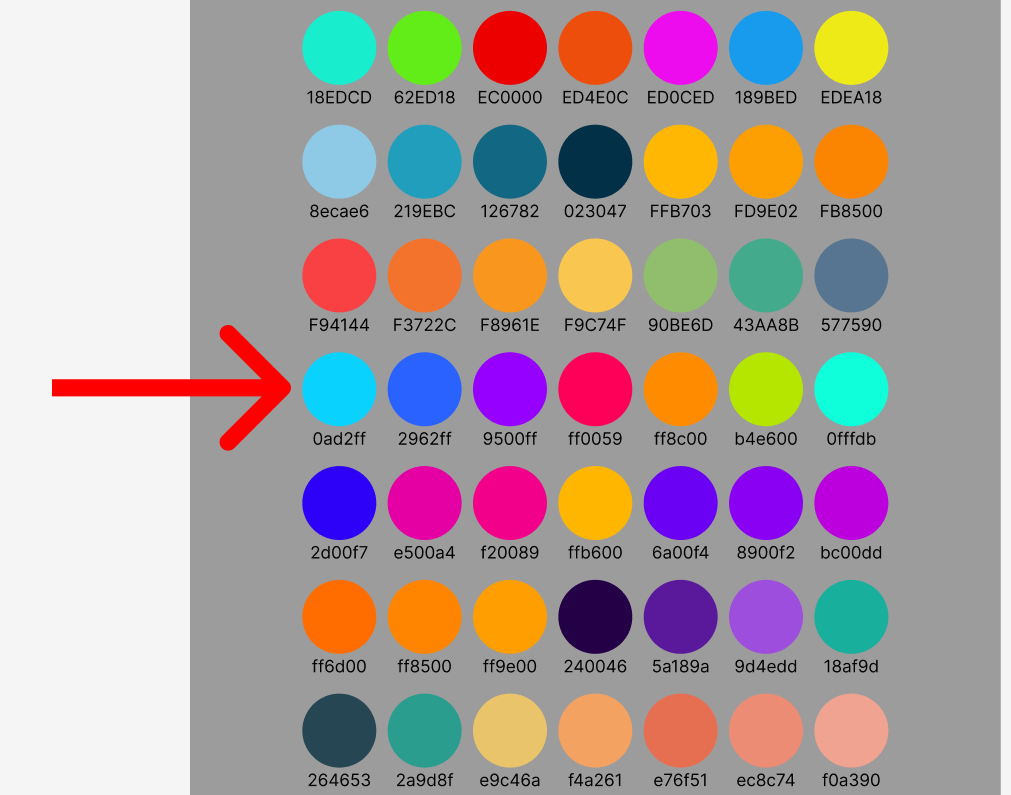
\includegraphics[width=0.7\textwidth]{PaletaDeColorFN.png}%
\caption{Paleta de color de Friends Night}%
\label{PCFN}%
\end{figure}
%%
\section{Tipografia del juego}
\par Para los titulos, en especial el titulo principal se usará la letra "Bungee" que llama la atención de una manera no tan formal, dando esa sensación de un gran titulo de película, para letras normales como las instrucciones o en ajustes se usara la letra Inter, la cual es legible, simple y al no tener serifa da la sensación de informalidad que buscamos. Por último, específicamente para cuando se mencione nuestra marca (Cor Studios) se usará la letra Sansita One que tiene algunos elementos estilo cursiva y dan un toque hecho a mano. 
\bigskip

















%%%%%%%%%%%%%%%%%%%%%%%%%%%%%%%%%%%
\end{document}

